\chapter[Energia]{Energia}
\section[NoBreak]{NoBreak}
\subsection[Requisitos do Projeto]{Requisitos do Projeto}
    \subsubsection[Retificador]{Retificador}
        \textbf{Dado} que a concessionária de energia forneça tensão
        
        \textbf{E} a máquina esteja em funcionamento
        
        \textbf{Então} a tensão da bateria deve ser carregada 
        
    \subsubsection[Inversor]{Inversor}
        \textbf{Dado} que a bateria forneça tensão
        
        \textbf{E} a máquina esteja em funcionamento
        
        \textbf{Então} a maquina deve ter tensão de alimentação
        
\subsection[Projeto]{Projeto}     
    \subsubsection[Retificador]{Retificador}            
        O projeto do retificador do NoBreak tem o objetivo de carregar a bateria do 					dispositivo enquanto houver energia fornecida da concessionária. O retificador 				deve ser um circuito estável, mantendo o padrão de fornecer sempre a tensão de 				saída necessária para a carga (Bateria). Logo, os requisitos desse subproduto 					são:

        \begin{itemize}
            \item Tensão de entrada: $220V_{AC}$
            \item Tensão de saída: $12V_{DC}$
            \item Corrente mínima: $5A$
        \end{itemize}

        Atendendo a esses requisitou a proposta do projeto é um retificador linear com 				a corrente máxima fornecida a carga de 5A seguindo os seguintes passos:
        
        \begin{figure}[!htb]
            \centering
            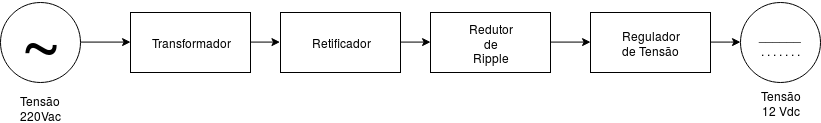
\includegraphics[scale= 0.5]{figuras/Diagrama_Retificador.png}
            \caption{Diagrama de blocos do Retificador. Fonte: Própria.}
            \label{diagrama-retificador}
        \end{figure}
        
        Para solucionar o que proposto, o primeiro passo foi calcular os parâmetros do 				circuito para suportar a corrente de 5A requisitada. A tensão do primário deve 				ser a tensão fornecida pela concessionária, no caso 220V. Para a tensão do 						secundário, deve-se utilizar a tensão de saída do circuito retificador, porém 					sabendo que o bloco retificador da figura 1 causa uma queda de tensão pequena, 				utilizou-se a tensão de secundário acima da necessária (12V). O valor 							comercial acima mais próximo para tensão de saída é de 16v. Para o 								transformador, necessitou-se o cálculo da potência dele.

            \begin{equation}
            S = V*I = 16*5 = 80VA
        \end{equation}
        
        Onde
        
        V = Tensão no secundário do transformador
        
        I = Corrente requisitada pelo projeto
        
        S = Potência complexa (Volt-Ampère)

        O transformador escolhido foi comprado pela internet com as exatas 								características propostas.

        \begin{figure}[!htb]
            \centering
            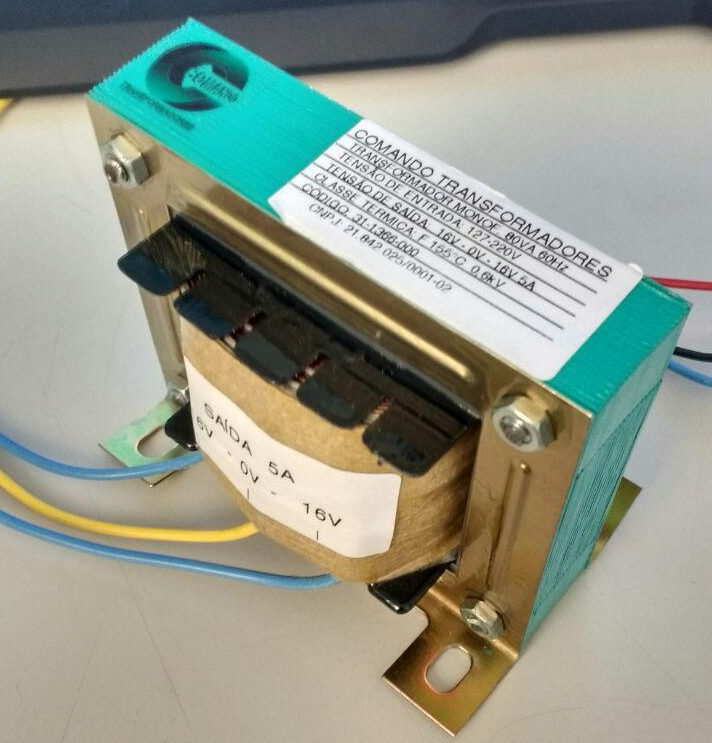
\includegraphics[scale= 0.3]{figuras/Transformador.png}
            \caption{Transformador do Retificador. Fonte: Própria.}
            \label{transformador-retificador}
        \end{figure}	
        
        O bloco Retificador escolheu-se um retificador de meia ponte devido ao 							transformador ter um enrolamento secundário com Tap central. O funcionamento 					deste bloco é ceifar o lado negativo da tensão alternada. 			

        \begin{figure}[!htb]
            \centering
            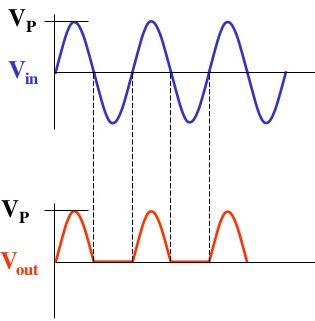
\includegraphics[scale= 0.5]{figuras/Retificador.png}
            \caption{Gráfico Tensão de entrada e saída de um diodo. Fonte: Própria.}
            \label{retificador}
        \end{figure}		
        
        Como são duas bobinas invertidas no secundário do transformador, uma bobina 					vai ceifar o lado negativo da tensão e a outra o lado positivo da tensão, ao 					somarem os dois resultados, o circuito resultante irá realizar o mesmo papel 					de um retificador de onda completa.
        
        O diodo retificador deve suportar a corrente máxima do projeto de 5A. Para 						isso, utilizou-se um diodo 6A10 que de acordo com o datasheet, a corrente 						máxima suportada é de 5A.
        
        Observa-se que a tensão resultante após o bloco retificador oscilará entre um 					pulso e outro de forma relevante. Essa oscilação denomina-se Ripple. Para 						deixar a tensão de saída mais linear possível, utiliza-se o bloco redutro de 					ripple. Este bloco  tem como função atrasar o tempo de carregamento da onda, 					fazendo com que no momento do descarregamento a saída deste bloco não consiga 					acompanhar, mantendo uma tensão mais estável. Para isso, utiliza-se um 							capacitor em paralelo com o circuito. O capacitor deve ser grande para atrasar 				a onda, logo utiliza-se capacitores eletrolíticos, e suportar a tensão de pico 				da onda (No caso no mínimo 16v) Para isso utilizou-se um capacitor de 1000uF e 				50v.

        \begin{figure}[!htb]
            \centering
            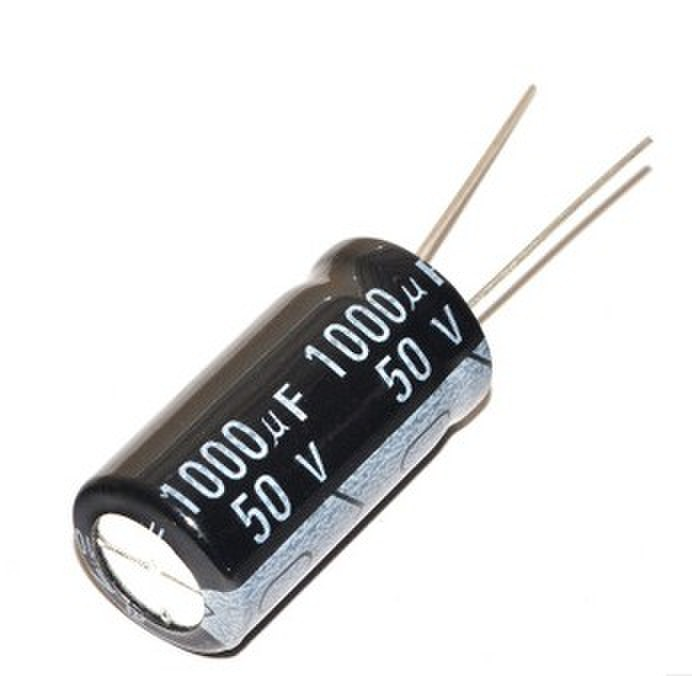
\includegraphics[scale= 0.2]{figuras/Capacitor.jpg}
            \caption{Capacitor redutor de Ripple. Fonte: Própria.}
            \label{capacitor}
        \end{figure}
        
        O bloco regulador de tensão tem a função de estabilizar a tensão para ficar o 					mais linear possível, porque para circuitos mais sensíveis a osicilação por 					menor que seja após o capacitor  pode ser prejudicial. Para realizar esta 						regulação, utiliza-se um diodo zener com a tensão zener exatamente na desejada 				para saída do projeto (No caso, 12v).  Para isso, utilizou-se um diodo zener 					4712A, cujo tensão zener é de 12v e a potência máxima é de 1w. Para proteção 					contra correntes invertida no circuito vinda da bateria, utilizou-se um diodo 					retificador 6A10 na saída do circuito no sentido da corrente convencional.

        O circuito completo do retificador foi simulado pelo software proteus e 						comprovado:
        
        \begin{figure}[!htb]
            \centering
            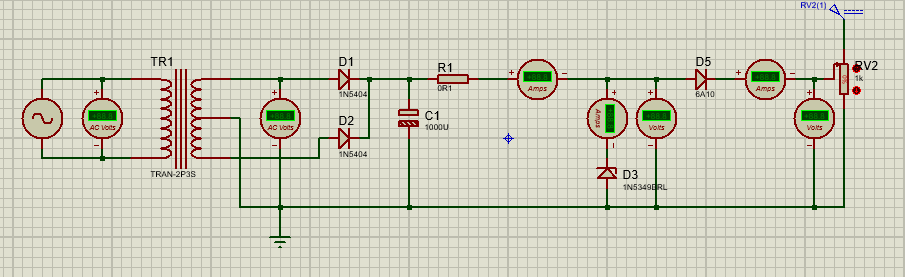
\includegraphics[scale= 0.4]{figuras/Circuito_Retificador.png}
            \caption{Simulação Retificador de tensão 12v. Fonte: Própria.}
            \label{retificador-completo}
        \end{figure}

     \subsubsection[Inversor]{Inversor}
        O projeto do inversor do NoBreak tem o objetivo de transformar a tensão 						contínua contida na bateria e transformá-la em tensão alternada para alimentar 				a carga . O inversor deve ser um circuito estável, mantendo o padrão de 						fornecer sempre a tensão de saída necessária para a carga (Máquina de Chopp). 					Logo, os requisitos desse subproduto são:
        
        \begin{itemize}
            \item Tensão de entrada: $12V_{DC}$
            \item Tensão de saída: $220V_{AC}$
            \item Corrente mínima: $3A$
        \end{itemize}
        
        Atendendo a esses requisitou a proposta do projeto é um inversor com a 							corrente máxima fornecida a carga de 4,5A seguindo os seguintes passos:
        
        \begin{figure}[!htb]
            \centering
            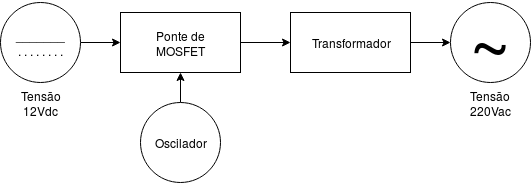
\includegraphics[scale= 0.4]{figuras/Diagrama_Inversor.png}
            \caption{Diagrama de blocos do Inversor. Fonte: Própria.}
            \label{diagrama-inversor}
        \end{figure} 
        Para solucionar o que proposto, o primeiro passo foi calcular os parâmetros do 				circuito para suportar a corrente de 4,5A requisitada. A tensão do primário 					deve ser a tensão da bateria, no caso 12v. Para a tensão do secundário, deve-					se utilizar a tensão que a carga necessita, neste caso 220Vac,. Para o 							transformador, necessitou-se o cálculo da potência dele.    
        
        \begin{equation}
            S = V*I = 220*4,5 = 1kVA
        \end{equation}
        
        Onde	
        
        V = Tensão no secundário do transformador
        
        I = Corrente requisitada pelo projeto

        S = Potência complexa (Volt-Ampère)
        
        O transformador escolhido foi fabricado com as exatas características 							propostas.		

        \begin{figure}[!htb]
            \centering
            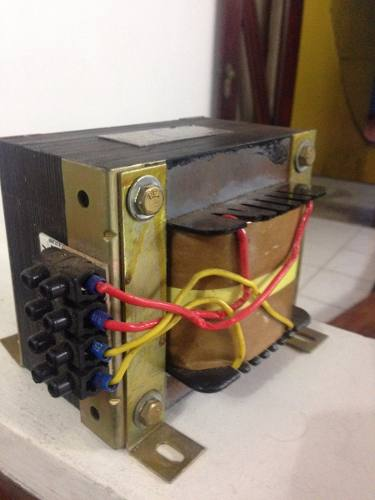
\includegraphics[scale= 0.3]{figuras/Transformador_Inversor.jpg}
            \caption{Transformador do inversor. Fonte: Própria.}
            \label{transformador-inversor}
        \end{figure}  

        O bloco oscilador tem como função criar uma onda modelo para criar a tensão 					alternada. Essa onda modelo deve ter frequência de 60Hz assim como é na tensão 				utilizada pela concessionária de energia. O primeiro teste de oscilador foi 					com um circuito oscilador a partir de um CI 4047. Esse CI tem a função de 						alternar entre uma saída e outra uma tensão na frequência determinada por uma 					equivalência entre resistor e capacitor na entrada do CI. Ao fazerem testes 					observou-se que a tensão de saída em uma das portas oscilava com a frequência 					duas vezes maior que a frequência na outra porta. A conclusão tirada desses 					testes é que o CI estava com defeito, porém por falta de tempo, adotou-se 						outra solução mais rápida.
        
        A segunda solução aplicada foi realizar um circuito oscilado a partir de um 					microcontrolador. O controlador escolhido foi um AtTiny por ser pequeno, 						econômico e rápido o suficiente para esta aplicação. O programa compilado nele 				faz a função de escrever nível lógico alto em uma porta, aguardar 16,6ms 						(Aproximadamente 60Hz) escrever nível lógico baixo nesta porta e o inverso com 				outra porta. 	

        \begin{figure}[!htb]
            \centering
            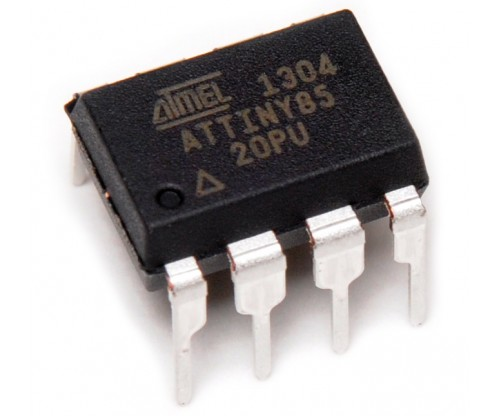
\includegraphics[scale= 0.2]{figuras/Attiny.jpg}
            \caption{Attiny 85. Fonte: Própria.}
            \label{attiny}
        \end{figure} 	
        
        A saída da etapa do oscilador é utilizada pelo bloco de ponte de MosFet. A 						ponte de MosFet tem a função de amplificar a onda gerada pelo oscilador além 					de ser capaz de suportar quantidades grandes de corrente. O MosFet escolhido 					para este projeto é o IRF2807, de acordo com o datasheet, o componente é capaz 				de suportar corrente de dreno de até 75A.	
        
        \begin{figure}[!htb]
            \centering
            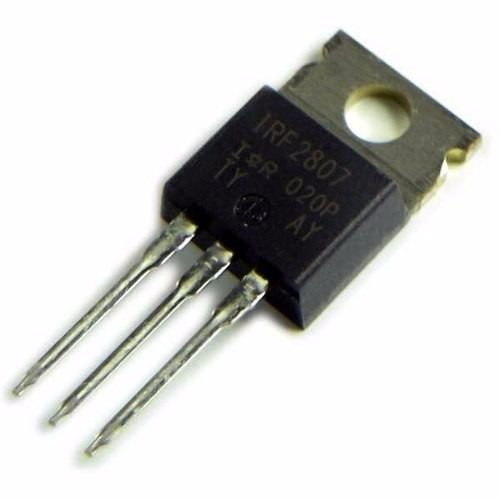
\includegraphics[scale= 0.2]{figuras/IRF2807.jpg}
            \caption{MosFet IRF2807. Fonte: Própria.}
            \label{mosfet}
        \end{figure}            						
        
        Após a ponte de MosFet o circuito passa pelo transformador e filtro RLC para 					alcançar o mais próximo de uma senóide com tensão RMS de 220v. O filtro RLC 					foi projetado para o circuito abaixo:	

        \begin{figure}[!htb]
            \centering
            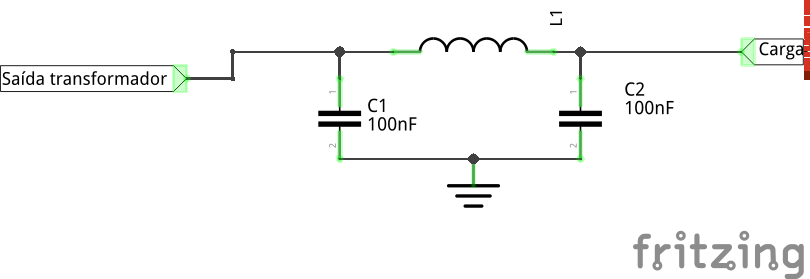
\includegraphics[scale= 1.0]{figuras/Filtro_RLC.png}
            \caption{Filtro RLC. Fonte: Própria.}
            \label{rlc}
        \end{figure}  				
        
        O filtro apesar de ser RLC, conta apenas com indutor e capacitor, pois a 						resistência do circuito é a própria resistência do indutor.
        
        O circuito todo projetado foi simulado de acordo com a imagem abaixo:
        
        \begin{figure}[!htb]
            \centering
            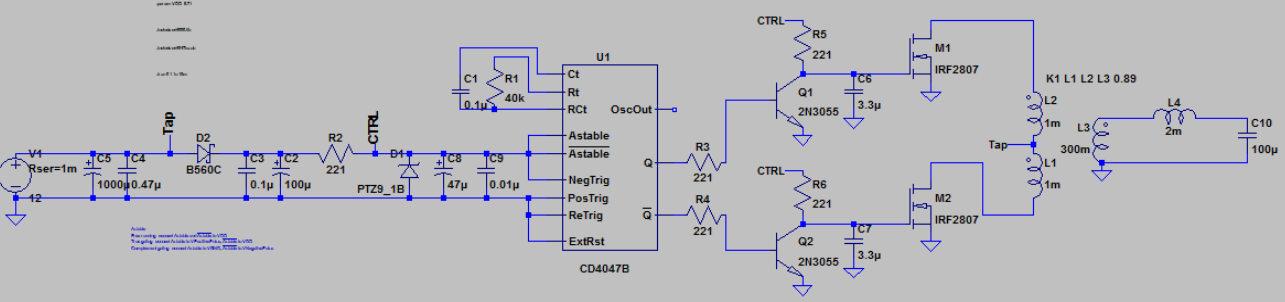
\includegraphics[scale= 0.4]{figuras/Circuito_inversor.png}
            \caption{Circuito inversor completo. Fonte: Própria.}
            \label{inversor}
        \end{figure} 
                        
        Alguns componentes como mostra a figura acima estão diferentes dos projetados 					pois no simulador não havia igual, mas foi pego o componente mais próximo para 				ser o mais próximo do real.          
     
\subsection[Solução Adotada]{Solução Adotada}
    \subsubsection[Retificador]{Retificador} 
        A partir dos testes de simulação montou-se o circuito em placa de fenolite. O 					design foi feito no software Traxmakker e para fabricação fez o processo 						térmico e depois corrosão.	
        
        \begin{figure}[!htb]
            \centering
            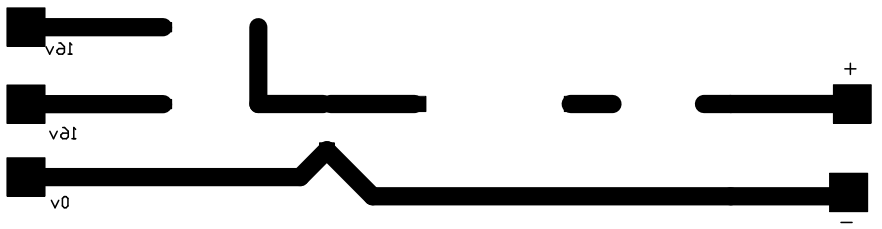
\includegraphics[scale= 0.4]{figuras/Fenolite_Retificador.png}
            \caption{Trilhas do circuito retificador. Fonte: Própria.}
            \label{retificador-fenolite}
        \end{figure}	
        
        \begin{figure}[!htb]
            \centering
            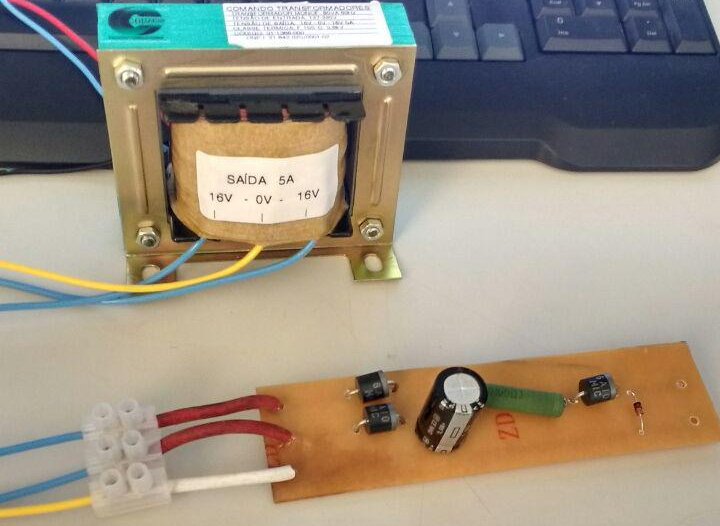
\includegraphics[scale= 0.4]{figuras/Circuito_Retificador_Completo.png}
            \caption{Circuito Retificador Completo. Fonte: Própria.}
            \label{retificador-completo2}
        \end{figure}	
        
        Para realizar a integração, o circuito retificador foi posicionado no 							local apresentado pela equipe de estrutura para o Nobreak. Na entrada do 						transformador adaptou-se a partir de um conector múltiplo um cabo PP $2,5mm^2$ 				de duas vias com um conector de tomada macho padrão ABNT 14136.             	

        \begin{figure}[!htb]
            \centering
            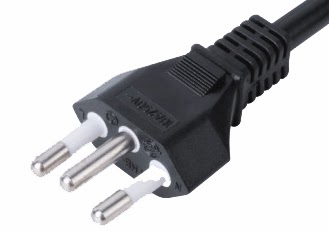
\includegraphics[scale= 0.4]{figuras/Pardrao_tomada.jpg}
            \caption{Tomada macho padrão ABNT. Fonte: Própria.}
            \label{tomada}
        \end{figure}	 
        
        Para saída do retificador adaptadou-se um cabo $6mm^2$ com um terminal de 						bateria automotiva universal para poder ter fácil acesso de tirar e 							colocar a bateria em caso de transporte ou manutenção.  
        
        \begin{figure}[!htb]
            \centering
            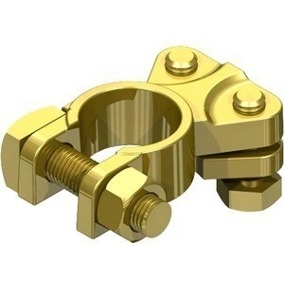
\includegraphics[scale= 0.4]{figuras/Terminal_Bateria.jpg}
            \caption{Terminal universal Bateria. Fonte: Própria.}
            \label{terminal}
        \end{figure}

        Notou-se que a corrente do circuito feito em testes estava limitada, e o 						componente que realiza este efeito é a resistência em série do circuito. Com 					isso, foi decidido em diminuir o valor resistivo o suficiente para deixar 						próximo ao máximo de potência dissipada. O valor do resistor que chegou 						próximo ao desejado foi $12\Omega$ e $10W$. A corrente máxima que o resistor 					passará é:
        
            \begin{equation}
            I = \frac{P}{V} = \frac{10}{12} = 0,833A
        \end{equation}            	
        
        A corrente máxima de 830mA é o suficiente para o projeto visto que a bateria 					não estará sobre carga a todo momento.

     \subsubsection[Inversor]{Inversor}            
        Para a fabricação da placa me fenolite atentou-se aos pontos em que a corrente 				será alta fazendo trilhas largas com capacidade para suportar a corrente 						necessária.

        \begin{figure}[!htb]
            \centering
            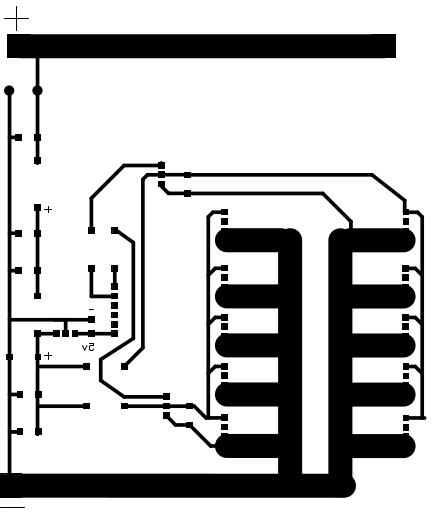
\includegraphics[scale= 0.4]{figuras/Placa_inversor.png}
            \caption{Placa impressa do inversor. Fonte: Própria.}
            \label{inversor-projeto}
        \end{figure} 		

        Percebe-se pelo circuito impresso que foram utilizados 5 mosfets para cada 						canal em paralelo. Colocar os Mosfets em paralelo faz com que a corrente por 					cada componente seja menor, aumentando a vida útil do componente e evitando 					que esquente excessivamente o sistema. Para cada canal de Mosfet será 							utilizado um dissipador de calor para melhorar a troca de calor do componente 					com o ambiente.		

        \begin{figure}[!htb]
            \centering
            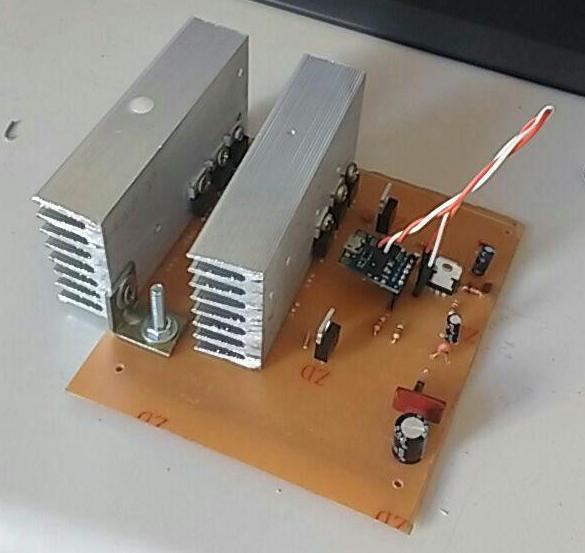
\includegraphics[scale= 0.4]{figuras/Inversor_pronto.jpg}
            \caption{Circuito inversor no circuito impresso. Fonte: Própria.}
            \label{inversor-pronto}
        \end{figure} 		
        
        De acordo com a figura acima, a saída do oscilador está em amarelo tem tensão 					de saída de 3,4v e frequência de 59,82Hz. O mesmo canal amplificado pelo 						MosFet apresenta a mesma frequência porém com tensão de 12,6v. 
        
        Para evitar a queima dos Mosfets, o oscilador não pode ter em nenhum momento 					os dois canais ligados, pois isso gera um curto circuito, queimando assim os 					mosfets. Para resolver este problema utilizou-se de um recurso chamado Tempo 					morto. Este tempo morto é um tempo no qual as duas portas do oscilador ficam 					destivadas para não haver curto entre os mosfets. Este tempo foi programado no 				Attiny e será ajustado quando houver integralização entre os projetos.           
        
        \begin{figure}[!htb]
            \centering
            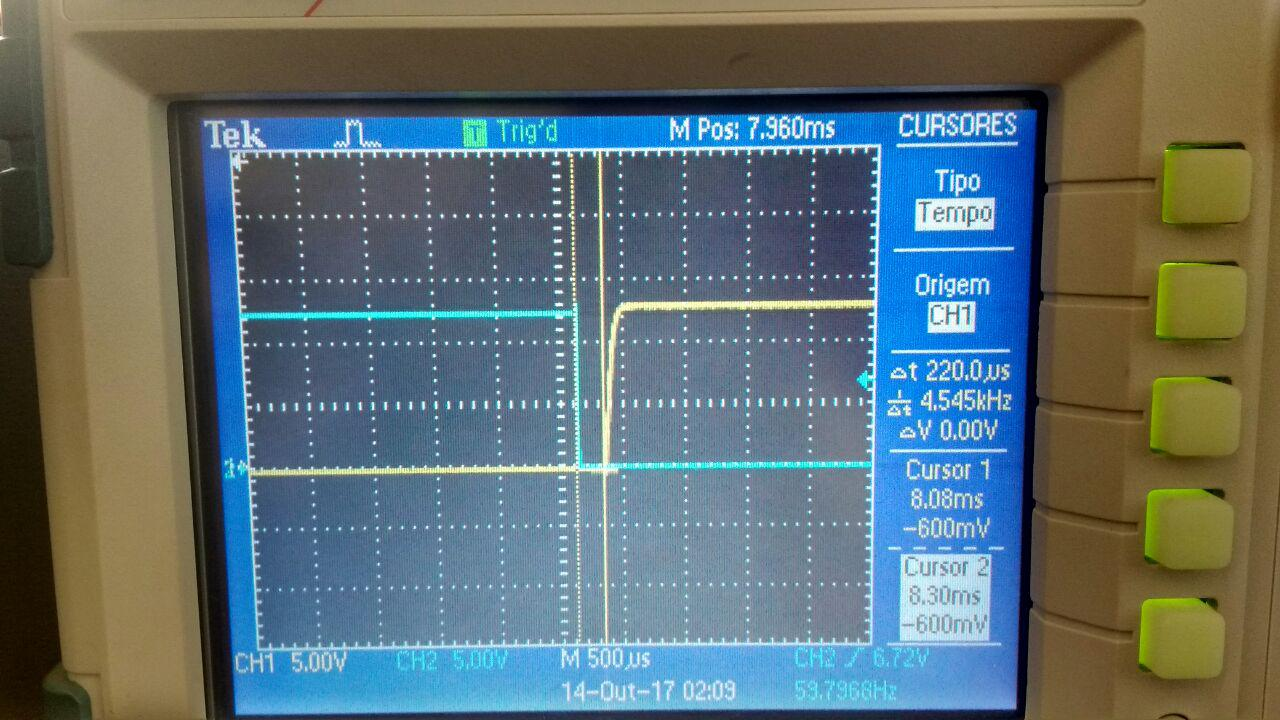
\includegraphics[scale= 0.2]{figuras/Tempo_morto.jpg}
            \caption{Tempo morto em testes. Fonte: Própria.}
            \label{tempo-morto}
        \end{figure}


\subsection[Casos de Teste]{Casos de Teste}
    \subsubsection[Retificador]{Retificador}       
       Os primeiros testes mostraram que o circuito funcionou, porém a corrente 						máxima que o retificador forneceu foi cerca de $90mA$. Com essa corrente o 						Nobreak teria dificuldade para carregar a bateria, não sendo eficiente em caso 				de falta de energia da concessionária. 
        
        \begin{figure}[!htb]
            \centering
            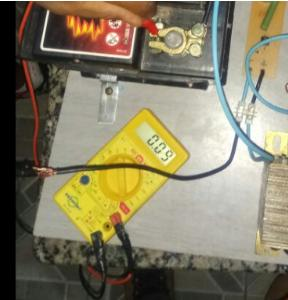
\includegraphics[scale= 0.6]{figuras/corrente_retificador.jpeg}
            \caption{Corrente primeiro teste no retificador. Fonte: Própria.}
            \label{corrente-retificador}
        \end{figure}            	
     
    \subsubsection[Inversor]{Inversor}
    
        A partir do circuito montado a saída do bloco da ponte de Mosfet em testes foi:
        
        \begin{figure}[!htb]
            \centering
            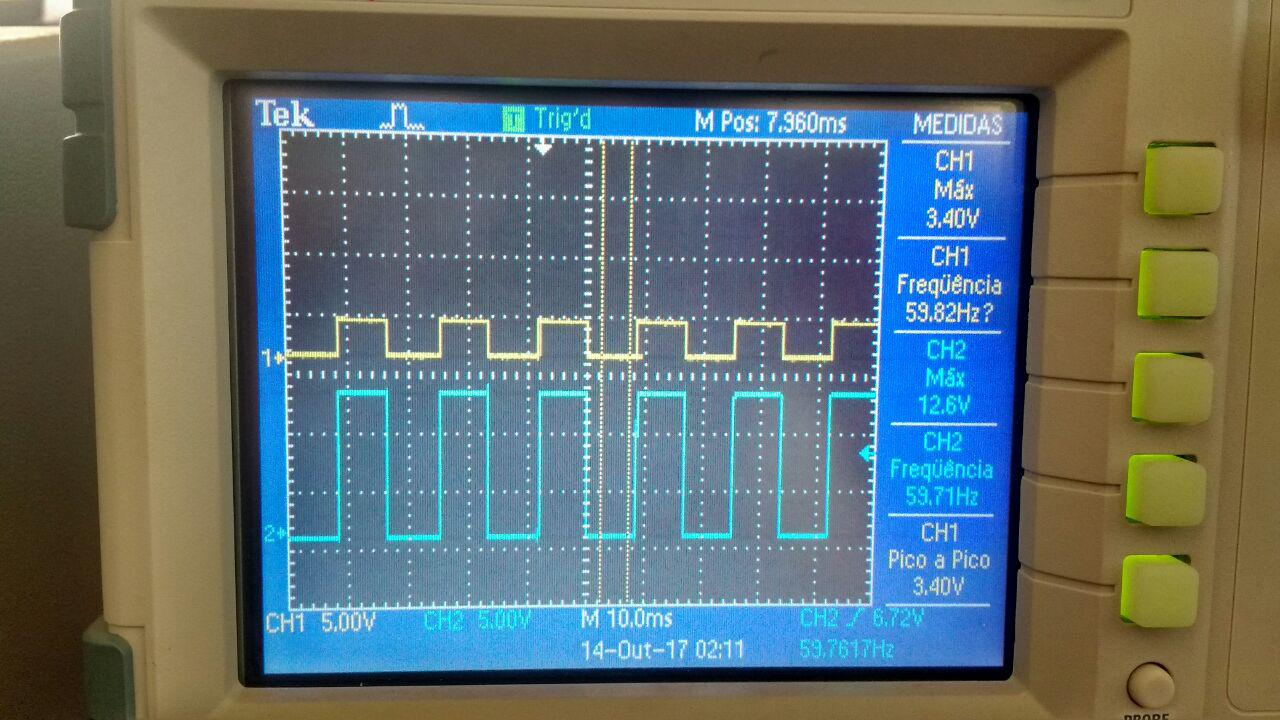
\includegraphics[scale= 0.2]{figuras/saida_inversor.jpg}
            \caption{Saída do bloco oscilador e ponte de MosFet. Fonte: Própria.}
            \label{saida-inversor}
        \end{figure}    

    \section[Sistema de Refrigeração]{Sistema de Refrigeração}
        \subsection[Requisitos do Projeto]{Requisitos do Projeto}
        
        \begin{itemize}
            \item \textbf{Dado} o sistema de refrigeração em funcionamento
            \item \textbf{E} um usuário solicitar chopp
            \item \textbf{Então} o chopp deve estar gelado pelo chirller para possibilitar o consumo
        \end{itemize}

        \subsection[Projeto]{Projeto}
            A demanda do problema exige que o Chopp seja resfriado de forma que o seu
            consumo seja agradável ao consumidor. Fundamentalmente, quando o usuário realiza
            a compra, e a máquina projetada deve fornecer Chopp gelado para que o usuario o
            consuma. Para solucionar essa demanda foi proposto uma arquitetura e montagem da
            máquina que seja responsável pelo resfriamento do fluido. O sistema constitui por um
            condensador, Chiller. Esse permite a passagem do fluido a ser refrigerado e em
            contato com o tubo ja em temperatura ideal para a troca de calor.

            O modelo abaixo uma visão inicial dos componentes presentes no sistema de
            refrigeracao

            IMAGEM 1

            O ciclo de refrigeração é um ciclo termodinâmico, no qual ocorre a retirada de calor de
            um ambiente. Esse ciclo é composto pelos seguintes itens: Evaporador, Compressor, Válvula
            de expansão e Condensador. O evaporador é um dispositivo que diminui a pressão do gás
            refrigerante, para que este diminua a temperatura e possa receber calor do ambiente a ser
            refrigerado. O compressor, por outro lado, irá comprimir o gás até a pressão do condensador,
            para que este condense e transfira o calor do gás para o ambiente, fazendo com que o gás
            fique no estado líquido e retorne ao ciclo. Primeiramente no processo de resfriamento ocorre a
            compressão isentrópica do fluido refrigerante pelo compressor. O gás percorre e segue para o
            condensador onde ocorre a transferência calor a pressão constante. Quando o fluido sai do
            condensador encaminha para a válvula isentrópico. E por fim, segue para o processo 4-1 onde
            há transferência de calor a pressão constante ao ambiente que deseja refrigerar \cite{boles}.

            O evaporador no ciclo anteriormente citado consiste em um trocador de calor.
            Trocadores de calor sao dispositivos complicados. O aumento da transferência de calor em
            trocadores de calor e’ geralmente acompanhado com o aumento de pressão e, assim, uma
            maior potência de bombeamento. Sendo assim, qualquer ganho na transferência de calor
            deverá ser ser ponderada em relação ao custo da queda de pressão que o acompanha \cite{boles}.

            A escolha para o trocador de calor do sistema escolheu-se o Chirller de contra fluxo.
            Essa escolha deveu-se ao fato de enquadrar o principio ativo requisitado para o resfriamento
            do chopp. O modelo de um chiller ideal e apresentado abaixo.

            IMAGEM 2

            O dimensionamento da potência do compressor, necessário no ciclo de
            refrigeração foi feito a partir da Primeira Lei da Termodinâmica,onde calculou-se a
            carga térmica necessária a ser retirada do chopp, considerando que a vazão
            necessária a ser retirada da chopeira é 45 l/h, ou aproximadamente, 0,00125$m^3$/s, a
            Primeira Lei para o compressor será:

            \begin{equation}
                Q_{(ponto)} = m_{(ponto)} \times (h_1 - h_2)
            \end{equation}

            Onde:
            \begin{itemize}
                \item Q = Quantidade de calor
                \item m = fluxo mássico (vazão multiplicada pela densidade)
                \item h = entalpia
            \end{itemize}

            Manipulando, têm-se:
            \begin{equation}
                h_1 - h_2 = Cp_{méd} \times (T_1 - T_2)
            \end{equation}

            Onde:
            \begin{itemize}
                \item $Cp_{médi}$ = Calor Específico a pressão constante
                \item T = Temperatura do fluido
            \end{itemize}
            então, substituindo na primeira equação teremos:
            
            \begin{equation}
                Q_{ponto} = m_{ponto} \times Cp_{méd} \times (T_1 - T_2)
            \end{equation}

            Consideramos como fluido para os cálculos a água, visto que o chopp possui
            grande concentração de água em sua composição e que não foram encontrados dados
            para o calor específico do chopp, a aproximação é aceitável. O valor de calor
            específico a pressão constante encontrado para a água é de 4,18KJ/Kg. A temperatura
            considerada na entrada do trocador de calor é a mesma que a temperatura ambiente
            de aproximadamente  25$^\circ$ C e a requerida na saída dele para estar de acordo com os
            requisitos é de aproximadamente 1$^\circ$ C Dessa forma, o fluxo mássico:

            \begin{equation}
                m_{ponto} = p \times V
            \end{equation}

            \begin{equation}
                m_{ponto} = 1000 \times 0,00125
            \end{equation}

            \begin{equation}
                m_{ponto} = 0,0125
            \end{equation}

            Logo, a carga térmica a ser retirada do fluido, no trocador de calor, pelo gás
            que sai do compressor será:

            \begin{equation}
                Q_{ponto} = 0.0125 \times 4.18 \times (25-(-1)) = 1.35 KW
            \end{equation}

            Por meios de análises de catálogos do fabricante, para a carga térmica
            precisaria de um compressor de $1 \over 2$ HP

            \subsubsection[Simulação do sistema de Refrigeração]{Simulação do sistema de Refrigeração}
                Para a segurança do funcionamento do sistema de refrigeração usou-se o
                Software CoolPack para a simulação do sistema como um todo. Nesse software dados
                construtivos físicos dos seguintes elementos foram inseridos: Evaporador,
                Condensador, moto-compressor e tubulação.
                
                A figura seguinte ilustra a simulação realizada no software juntamente com os os
                dados das temperaturas em cada estado. Essas temperaturas mostraram-se
                importantes para a confirmação que o sistema de refrigeração iria funcionar.

                \begin{figure}[!htb]
            		\centering
            		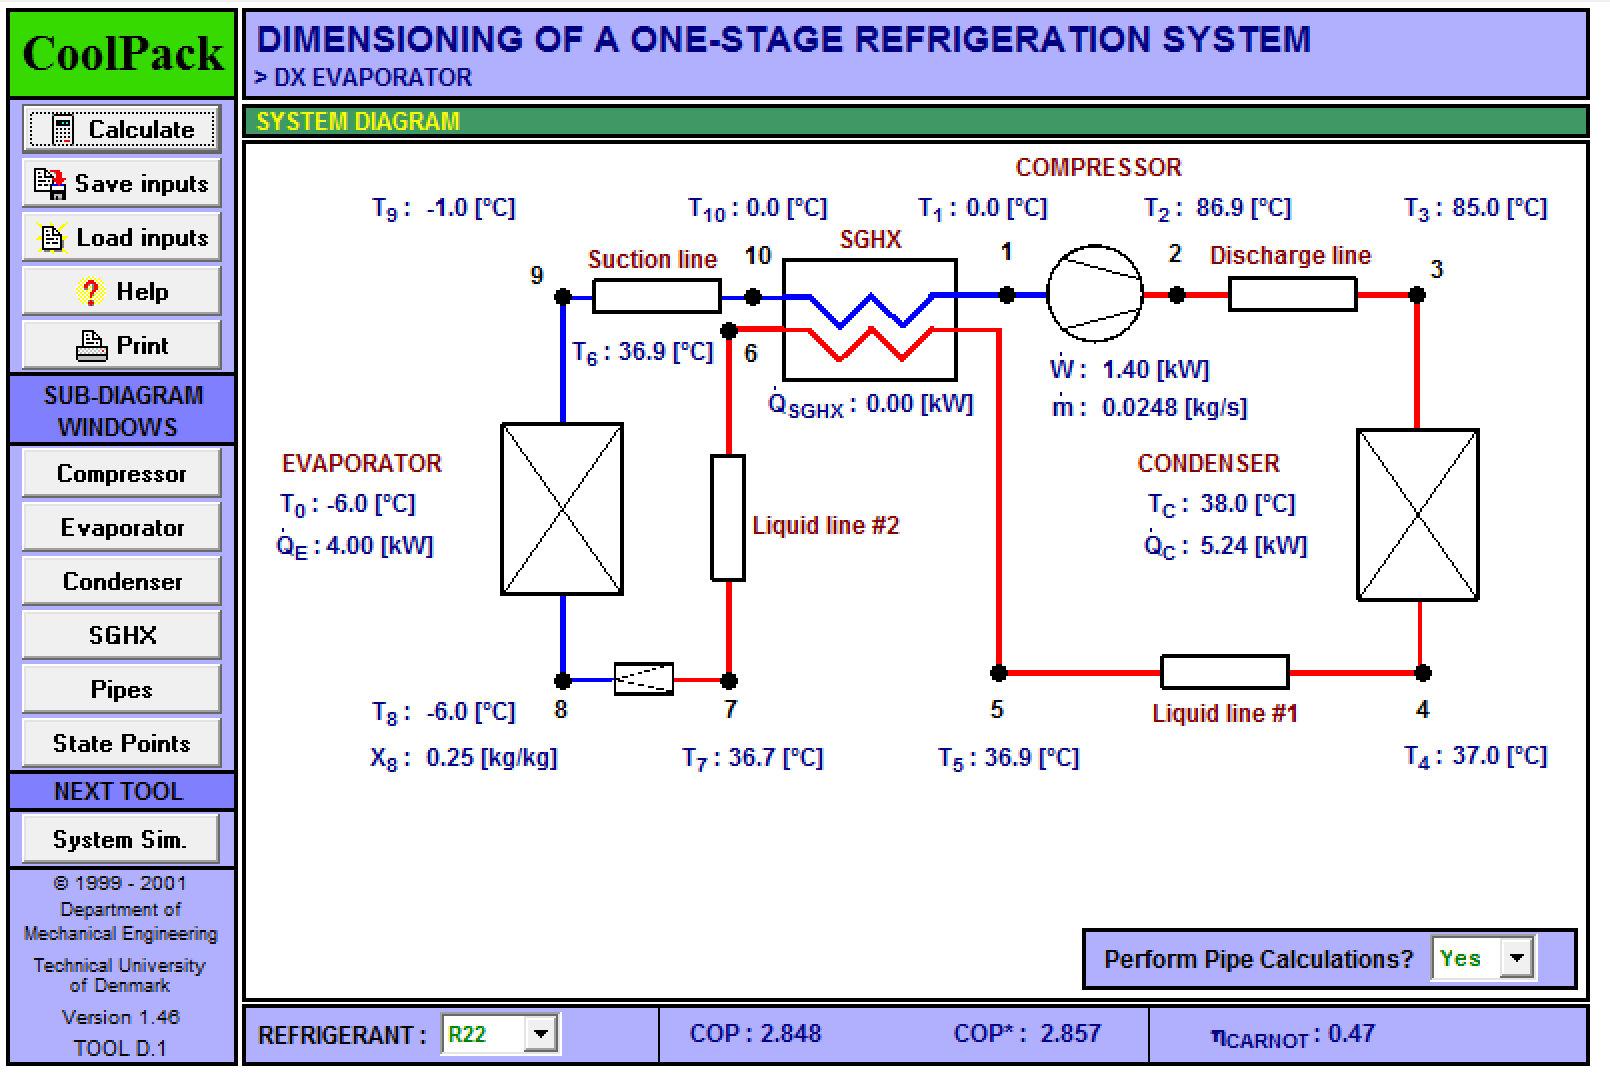
\includegraphics[scale= 0.3]{figuras/simulacao-refrigeracao.png}
            		\caption{Simulação do sistema de Refrigeração. Fonte: Própria.}
            		\label{simulacao-refrigeracao}
                \end{figure}
                
                Observa-se na imagem acima que foi inserido o dado correto quanto ao
                tipo de gás operante no compressor. Tem-se a quantidade calor transferida no
                evaporador que corresponde a 4.00 kW. Esse dado será validado nos testes do
                sistema já montado.
        
        \subsection[Casos de Teste]{Casos de Teste}
                \begin{itemize}
                    \item \textbf{Componente} Chiller
                    \item \textbf{Subsistema} Refrigeração
                    \item \textbf{Pré-condição} Haver Chopp gelado
                    \item \textbf{Entrada} Chopp quente
                    \item \textbf{Saída} Chopp gelado
                    \item \textbf{Fluxo de Eventos} Chopp quente entra em contra fluxo com o gás refrigerante a fim de
                        ter o chopp gelado.
                \end{itemize}

        \subsection[Solução Adotada]{Solução Adotada}
            \subsubsection[Montagem e Construção do Sistema de Refrigeração]{Montagem e Construção do Sistema de Refrigeração}
                A montagem foi feita com apenas um Chirller no protótipo por motivos de custo,
                sendo assim, a potência do compressor foi reduzida pela metade, ou seja, $1 \over 4$ Hp. O
                compressor foi cedido pelo professor Rander, para viabilizar que o protótipo fosse
                fabricado.
                
                Para a montagem do sistema de refrigeração teve que seguir as seguintes
                etapas:
                \begin{figure}[!htb]
            		\centering
            		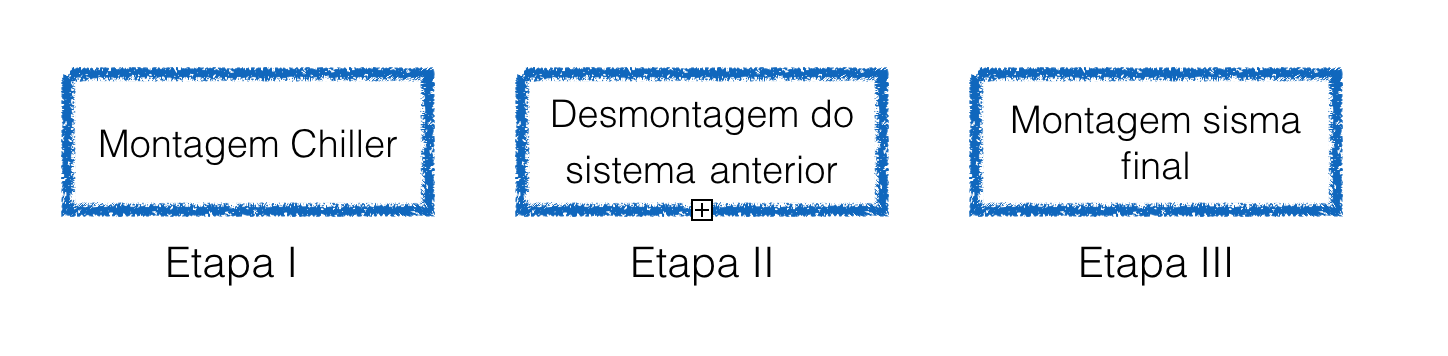
\includegraphics[scale= 0.3]{figuras/montagem-chiler.png}
            		\caption{Processo de Montagem do Sistema de Refrigeração. Fonte: Própria.}
            		\label{simulacao-refrigeracao}
                \end{figure}
                
                Neste processo, os materiais utilizados foram: uma panqueca de alumínio $3 \over 8$ e
                15 metros, uma mangueira atóxica trançada $3 \over 4$, 2 kits de engate rápido para
                mangueira, 2  reduções de $3 \over 4$ para $1 \over 2$, 2 tês de PVC com extremidades de $3 \over 4$
                e central de $1 \over 2$, 2 espigões de mangueira de $3 \over 4$ e 4 niples de união de $1 \over 2$,
                2 braçadeiras de $3 \over 4$ e 2 adaptadores de gás de $1 \over 2$ para $3 \over 8$.
                Primeiro, lavou-se a mangueira com água e sabão, feito isso,
                desenrolou-se a panqueca em todo o seu comprimento, de forma que ela
                ficasse bem reta. 
                
                Na segunda parte do processo, o tubo de alumínio foi inserido dentro da
                mangueira, ainda de forma que que a estrutura ficasse reta. Depois,
                enrolou-se a estrutura no molde, que tem 30cm de diâmetro, prendendo
                ele com lacres de plástico. A imagem a seguir ilustra esse processo,
                feito por membros do grupo:

                Foi feito um desenho esquemático do Chirller no software CatiaV5 para
                possibilitar as simulações, ele está ilustrado na figura \ref{desenho-chiller}.

                \begin{figure}[!htb]
                    \centering
                    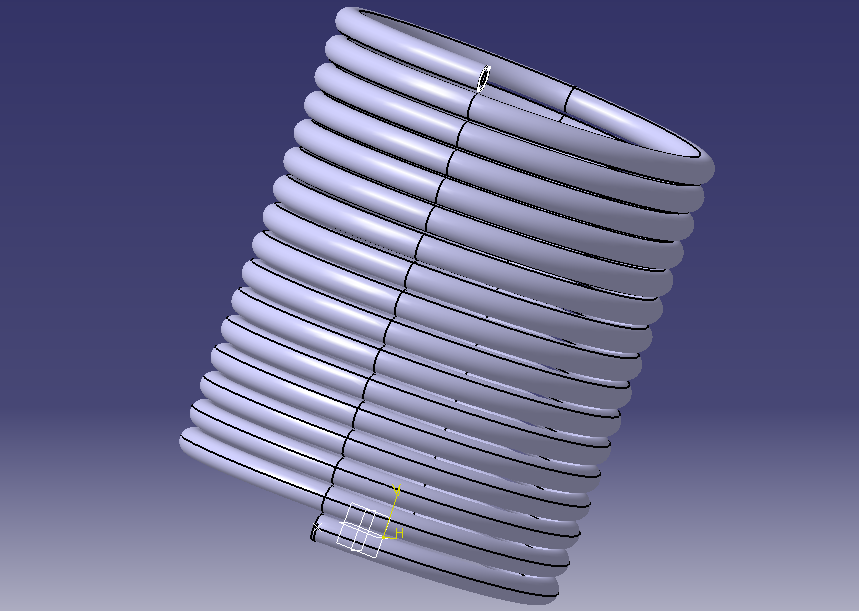
\includegraphics[scale= 0.3]{figuras/desenho-chiller.png}
                    \caption{Desenho esquemático do chirller. Fonte: Própria.}
                    \label{desenho-chiller}
                \end{figure}

                \begin{figure}[!htb]
                    \centering
                    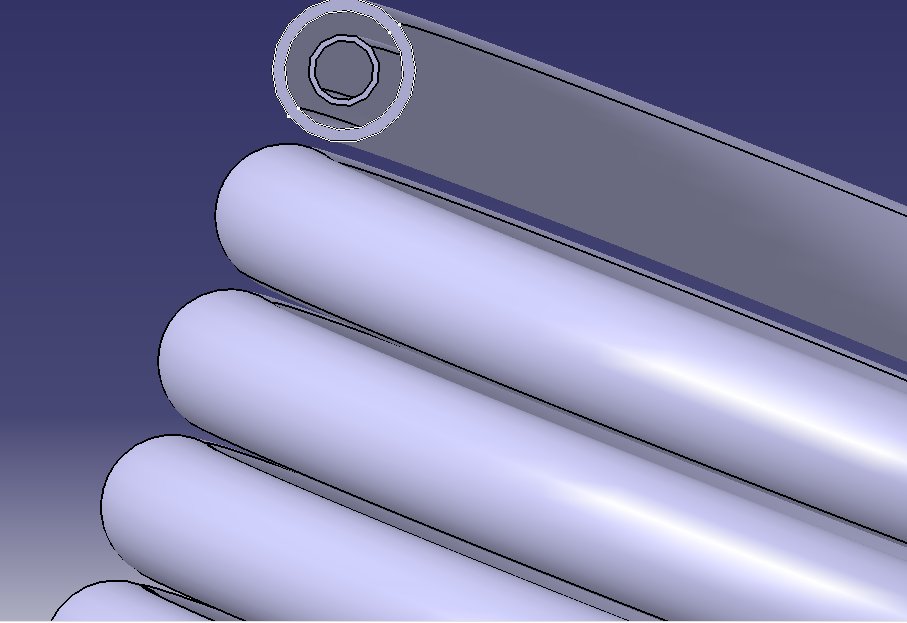
\includegraphics[scale= 0.3]{figuras/corte-mangeira.png}
                    \caption{Vista em corte da mangueira com o tubo de alumínio inserido. Fonte: Própria.}
                    \label{vista-mangueira}
                \end{figure}

                Na terceira parte da passagem, passou-se fita veda-rosca em todos os acessórios de
                tubulação, para evitar vazamentos, e montou-se o tê adaptado que possibilita a
                entrada e saída de chopp no Chirller de contra-fluxo. Neste processo,
                coloca-se o espigão em uma extremidade de $3 \over 4$ do tê, um nipple de união
                de $1 \over 2$ na extremidade de $1 \over 2$ do tê, um engate rápido no nipple. Na outra
                extremidade de $3 \over 4$, coloca-se uma redução de $3 \over 4$ pra $1 \over 2$, coloca-se
                um nipple de união e por fim, coloca-se um adaptador de gás no nipple. Depois
                de montado o tê adaptado ficou da seguinte maneira:

                \begin{figure}[!htb]
                    \centering
                    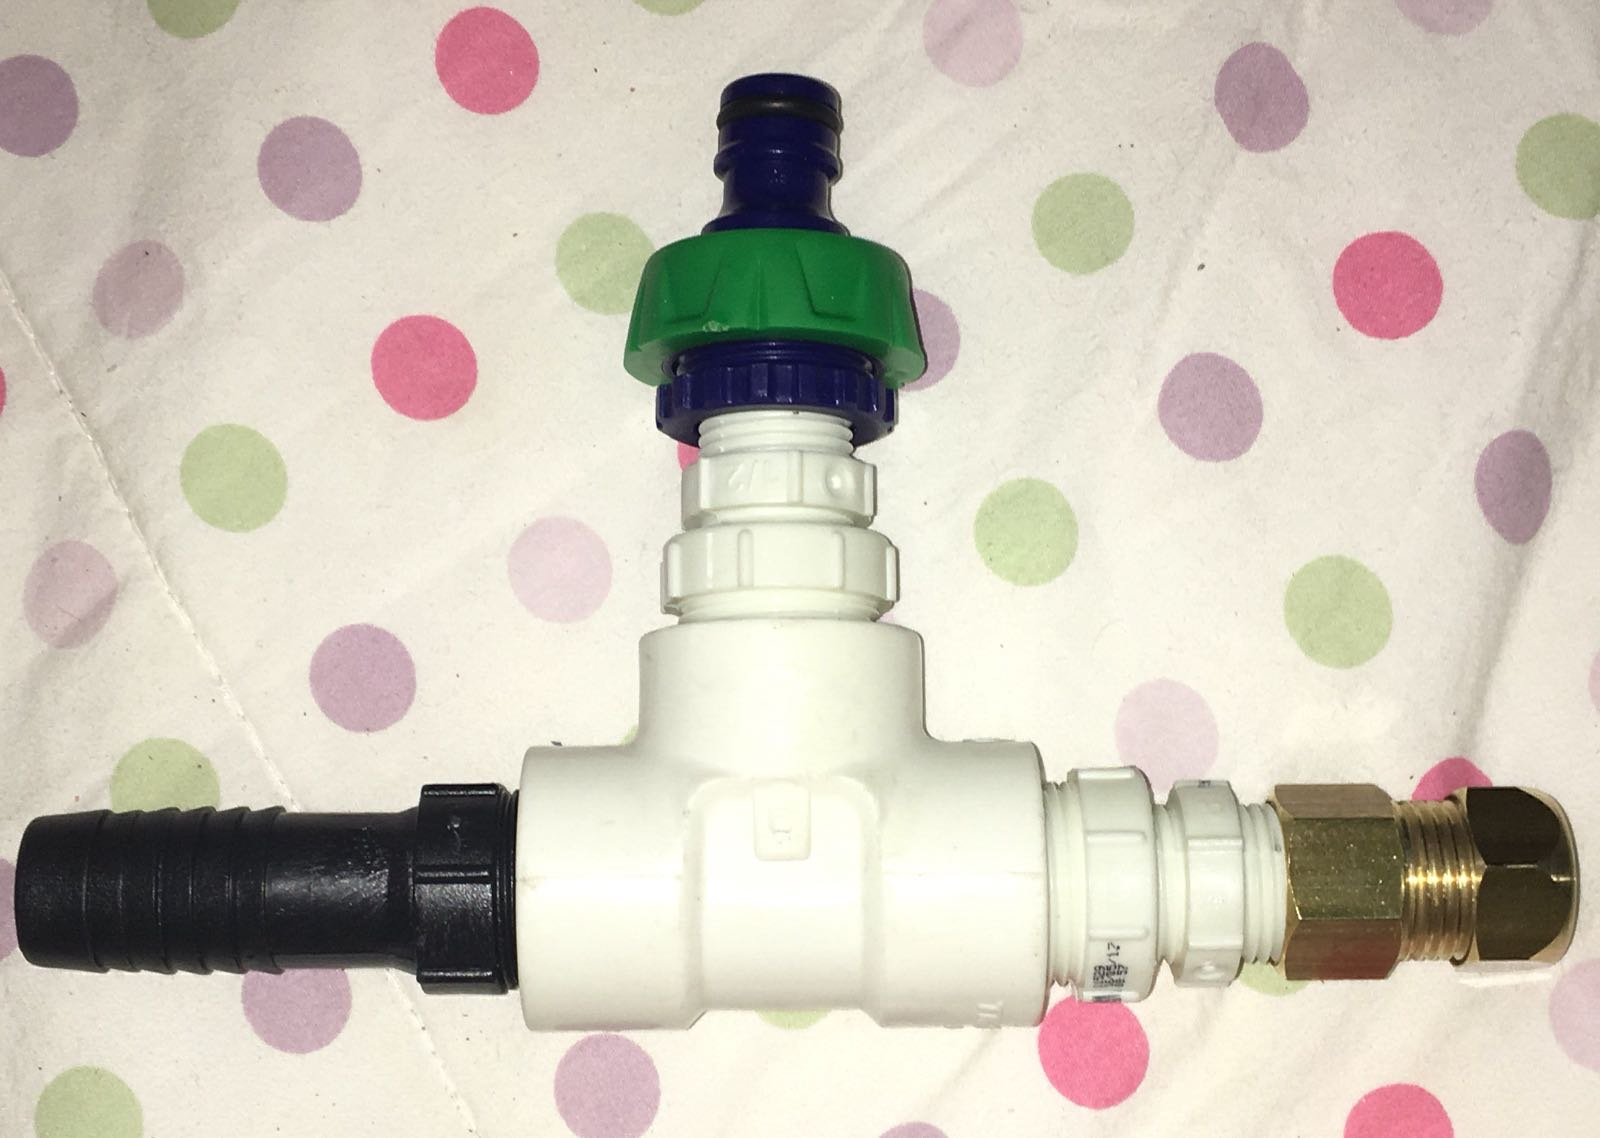
\includegraphics[scale= 0.3]{figuras/entrada-saida-chopp.png}
                    \caption{Tê adaptado para entrada e saída de chopp. Fonte: Própria.}
                    \label{entrada-saida-chopp}
                \end{figure}

                As peças todas foram compradas para montar dois tês, e conectar um a uma
                extremidade da mangueira e o outro a outra.

            \subsubsubsection[Desmontagem do Sistema]{Desmontagem do Sistema}
                Nessa etapa teve-se o devido cuidado para a desmontagem do sistema.
                Retirou-se o gás R22 com o equipamento próprio para tal ação, considerando assim a
                lei ambiental quanto a emissão de gases poluentes na atmosfera. Dessa forma, na
                válvula de serviço do compressor a válvula de descarga do fluido refrigerante
                encaminhando-o para o devido recipiente de armazenamento de gás a vacuo.
    
                Desse modo realizou-se o procedimento de recolhimento passivo. Esse
                procedimento e indicado para quantidades pequenas de gas. Ele pode ser retirado na
                sua forma gasosa ou líquida. Isso acontece devido a diferença de pressão entre os dois
                sistemas.

                Esse procedimento foi realizado a fim de atender a Resolução CONAMA no
                267, de 14 de setembro de 2000. Essa resolução proíbe a utilização e
                consequentemente emissão de substâncias que destroem a camada de ozônio.

            \subsubsubsection[Montagem do Sistema]{Montagem do Sistema}
                Após a devida manufatura do Chiller e a desmontagem do sistema escolheu-se
                uma base e alocou-se os componentes de acordo com a figura \ref{alocacao-dispositivos} 
                \begin{figure}[!htb]
                    \centering
                    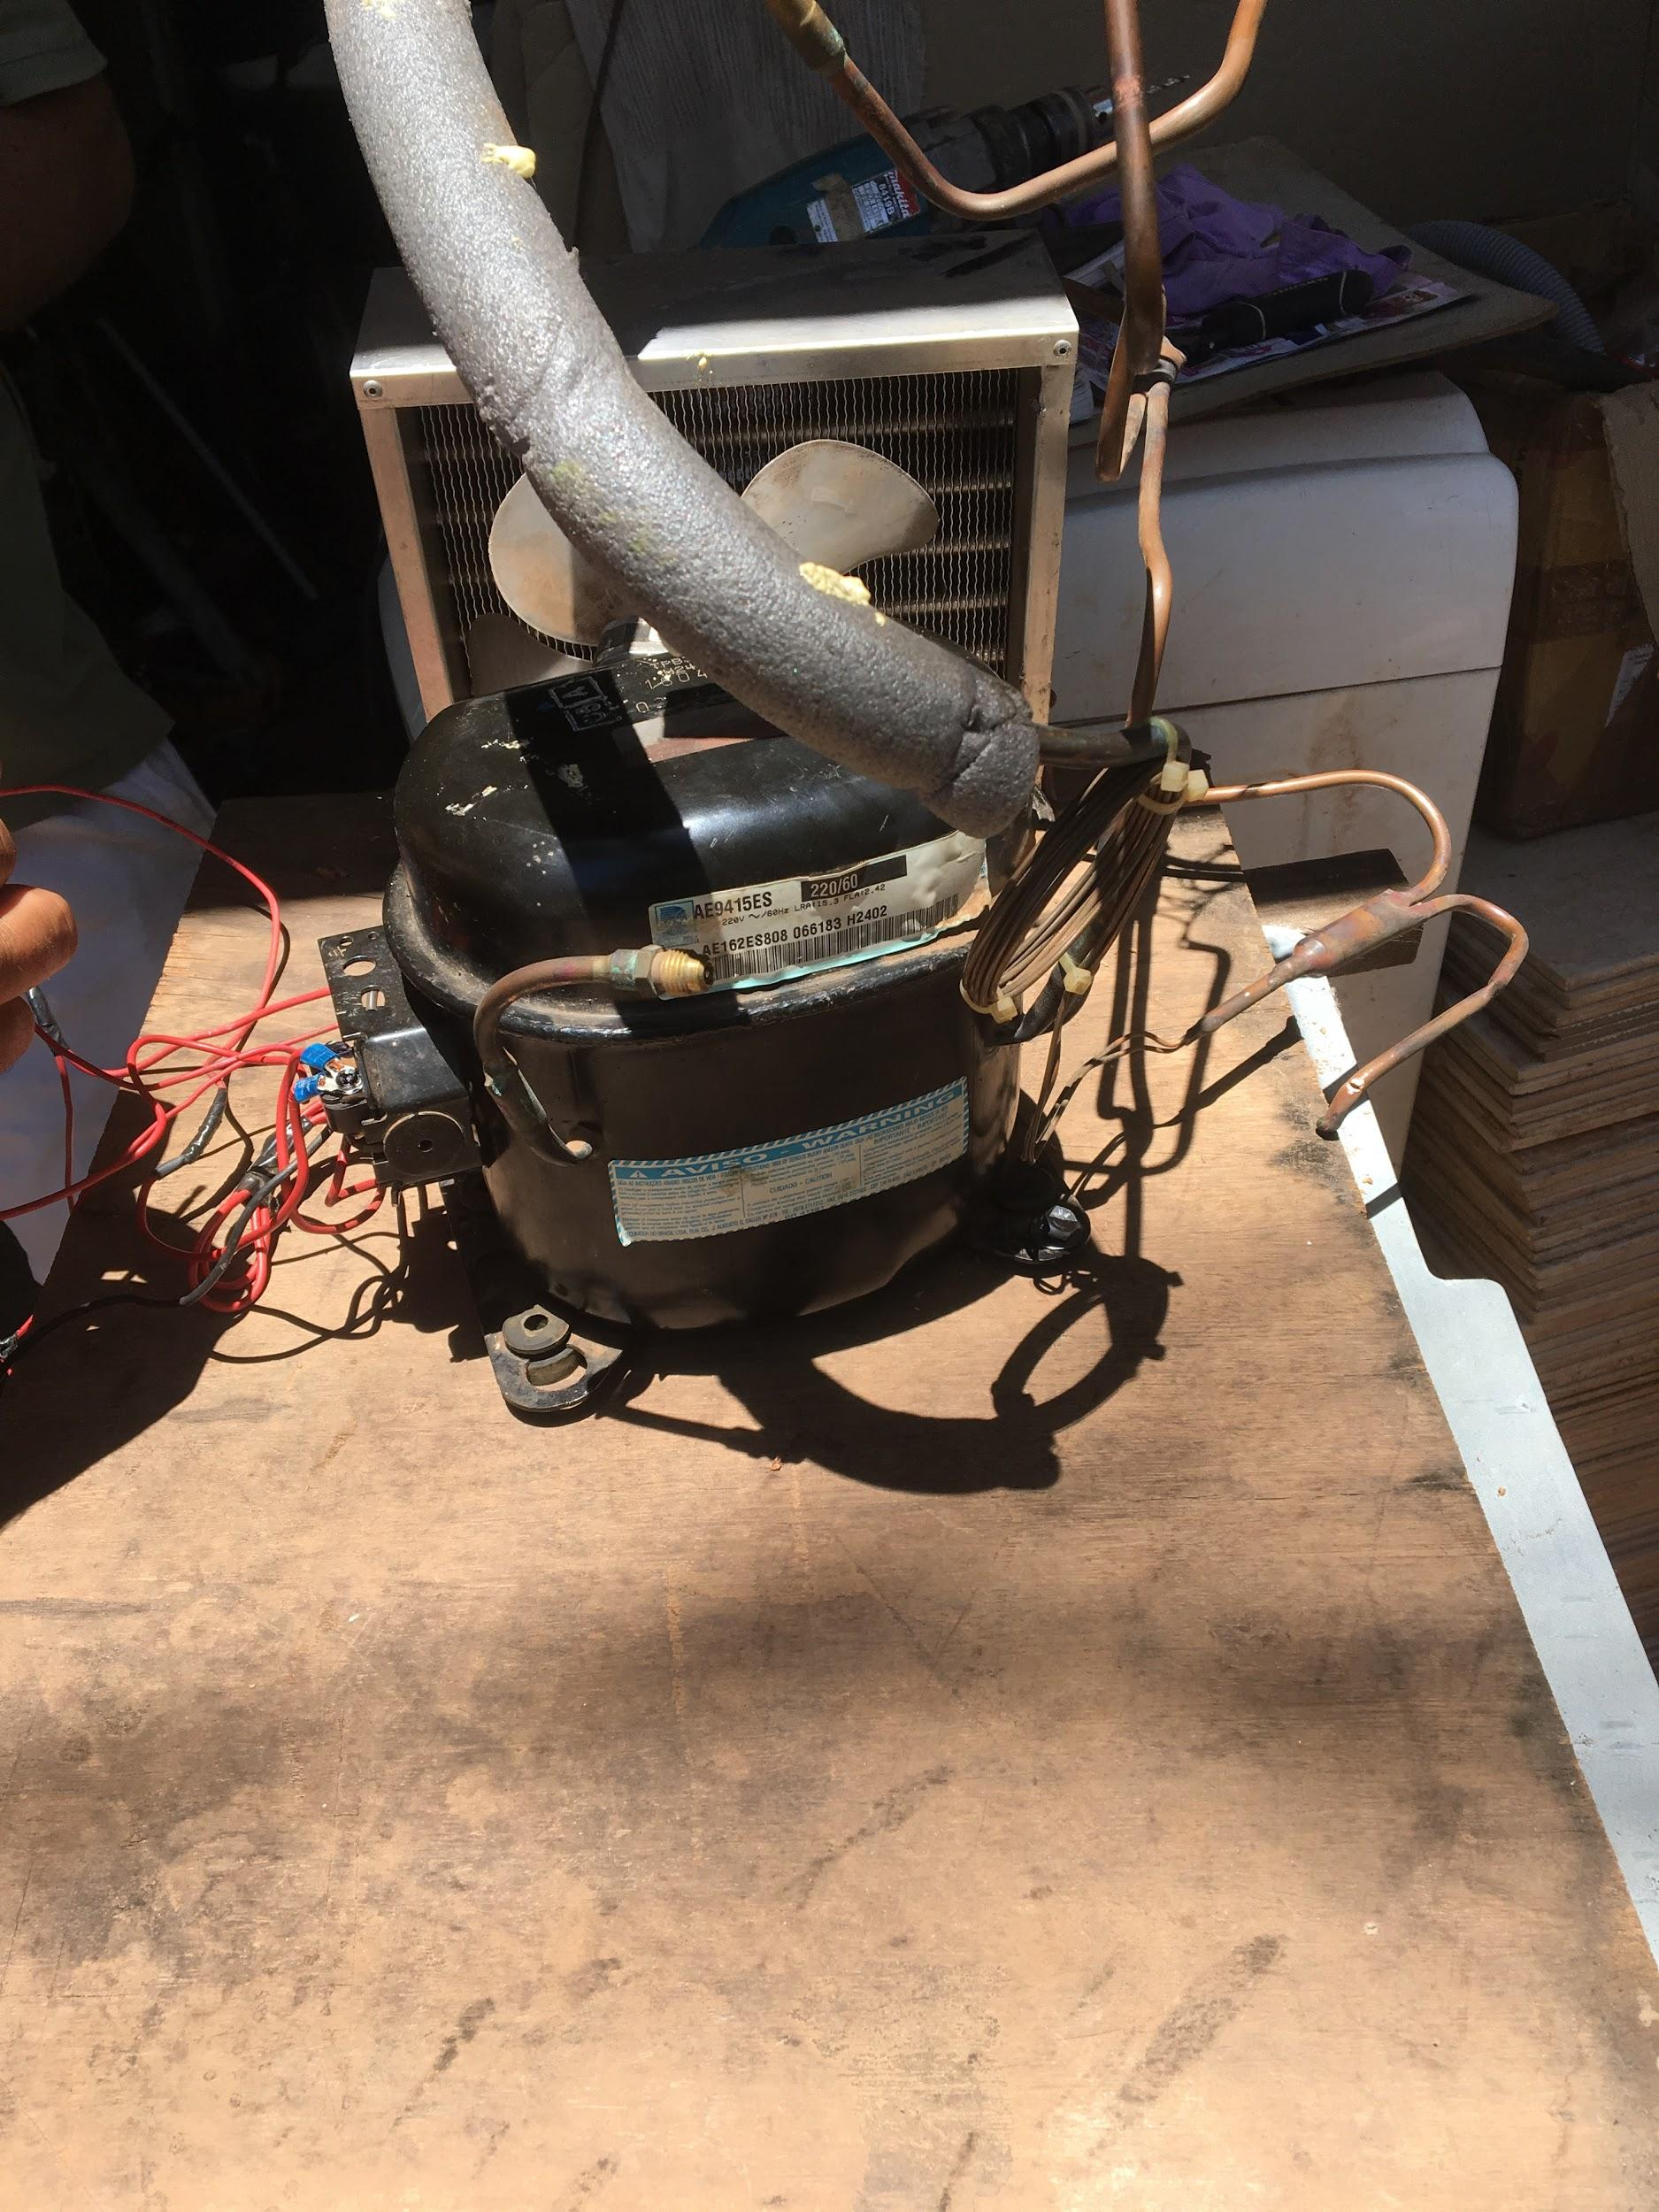
\includegraphics[scale= 0.2]{figuras/alocacao-dispositivos.png}
                    \caption{Sistema aberto e alocação dos dispositivos. Fonte: Própria.}
                    \label{alocacao-dispositivos}
                \end{figure}

                A base para o sistema consiste em uma de material madeira. Esse material foi
                escolhido devido às suas propriedades térmicas e pela fácil disponibilidade.
                
                Realizou-se testes de pressão no motocompressor e constatou-se que
                encontrava-se com baixa capacidade de compressão. Sendo assim realizou-se a
                limpeza do motor e também a troca de do filtro do sistema para o filtro secador do tipo
                Darfur. Este filtro impede com que partículas indesejadas passem pela a tubulação e
                cheguem no motocompressor. Além disso, como o filtro secador foi trocado optou-se,
                por medidas preventivas, trocar o filtro capilar.

                A tubulação do Chiller escolhido consiste de alumínio e as demais tubulações
                do sistema sao de cobre. Assim sendo, tornando inviável a solda desses dispositivos
                como solução. A partir disso, optou-se pela aquisição da junção de gás(nipel) com a
                cabeça em forma de cilindro ilustrado na figura abaixo.

                \begin{figure}[!htb]
                    \centering
                    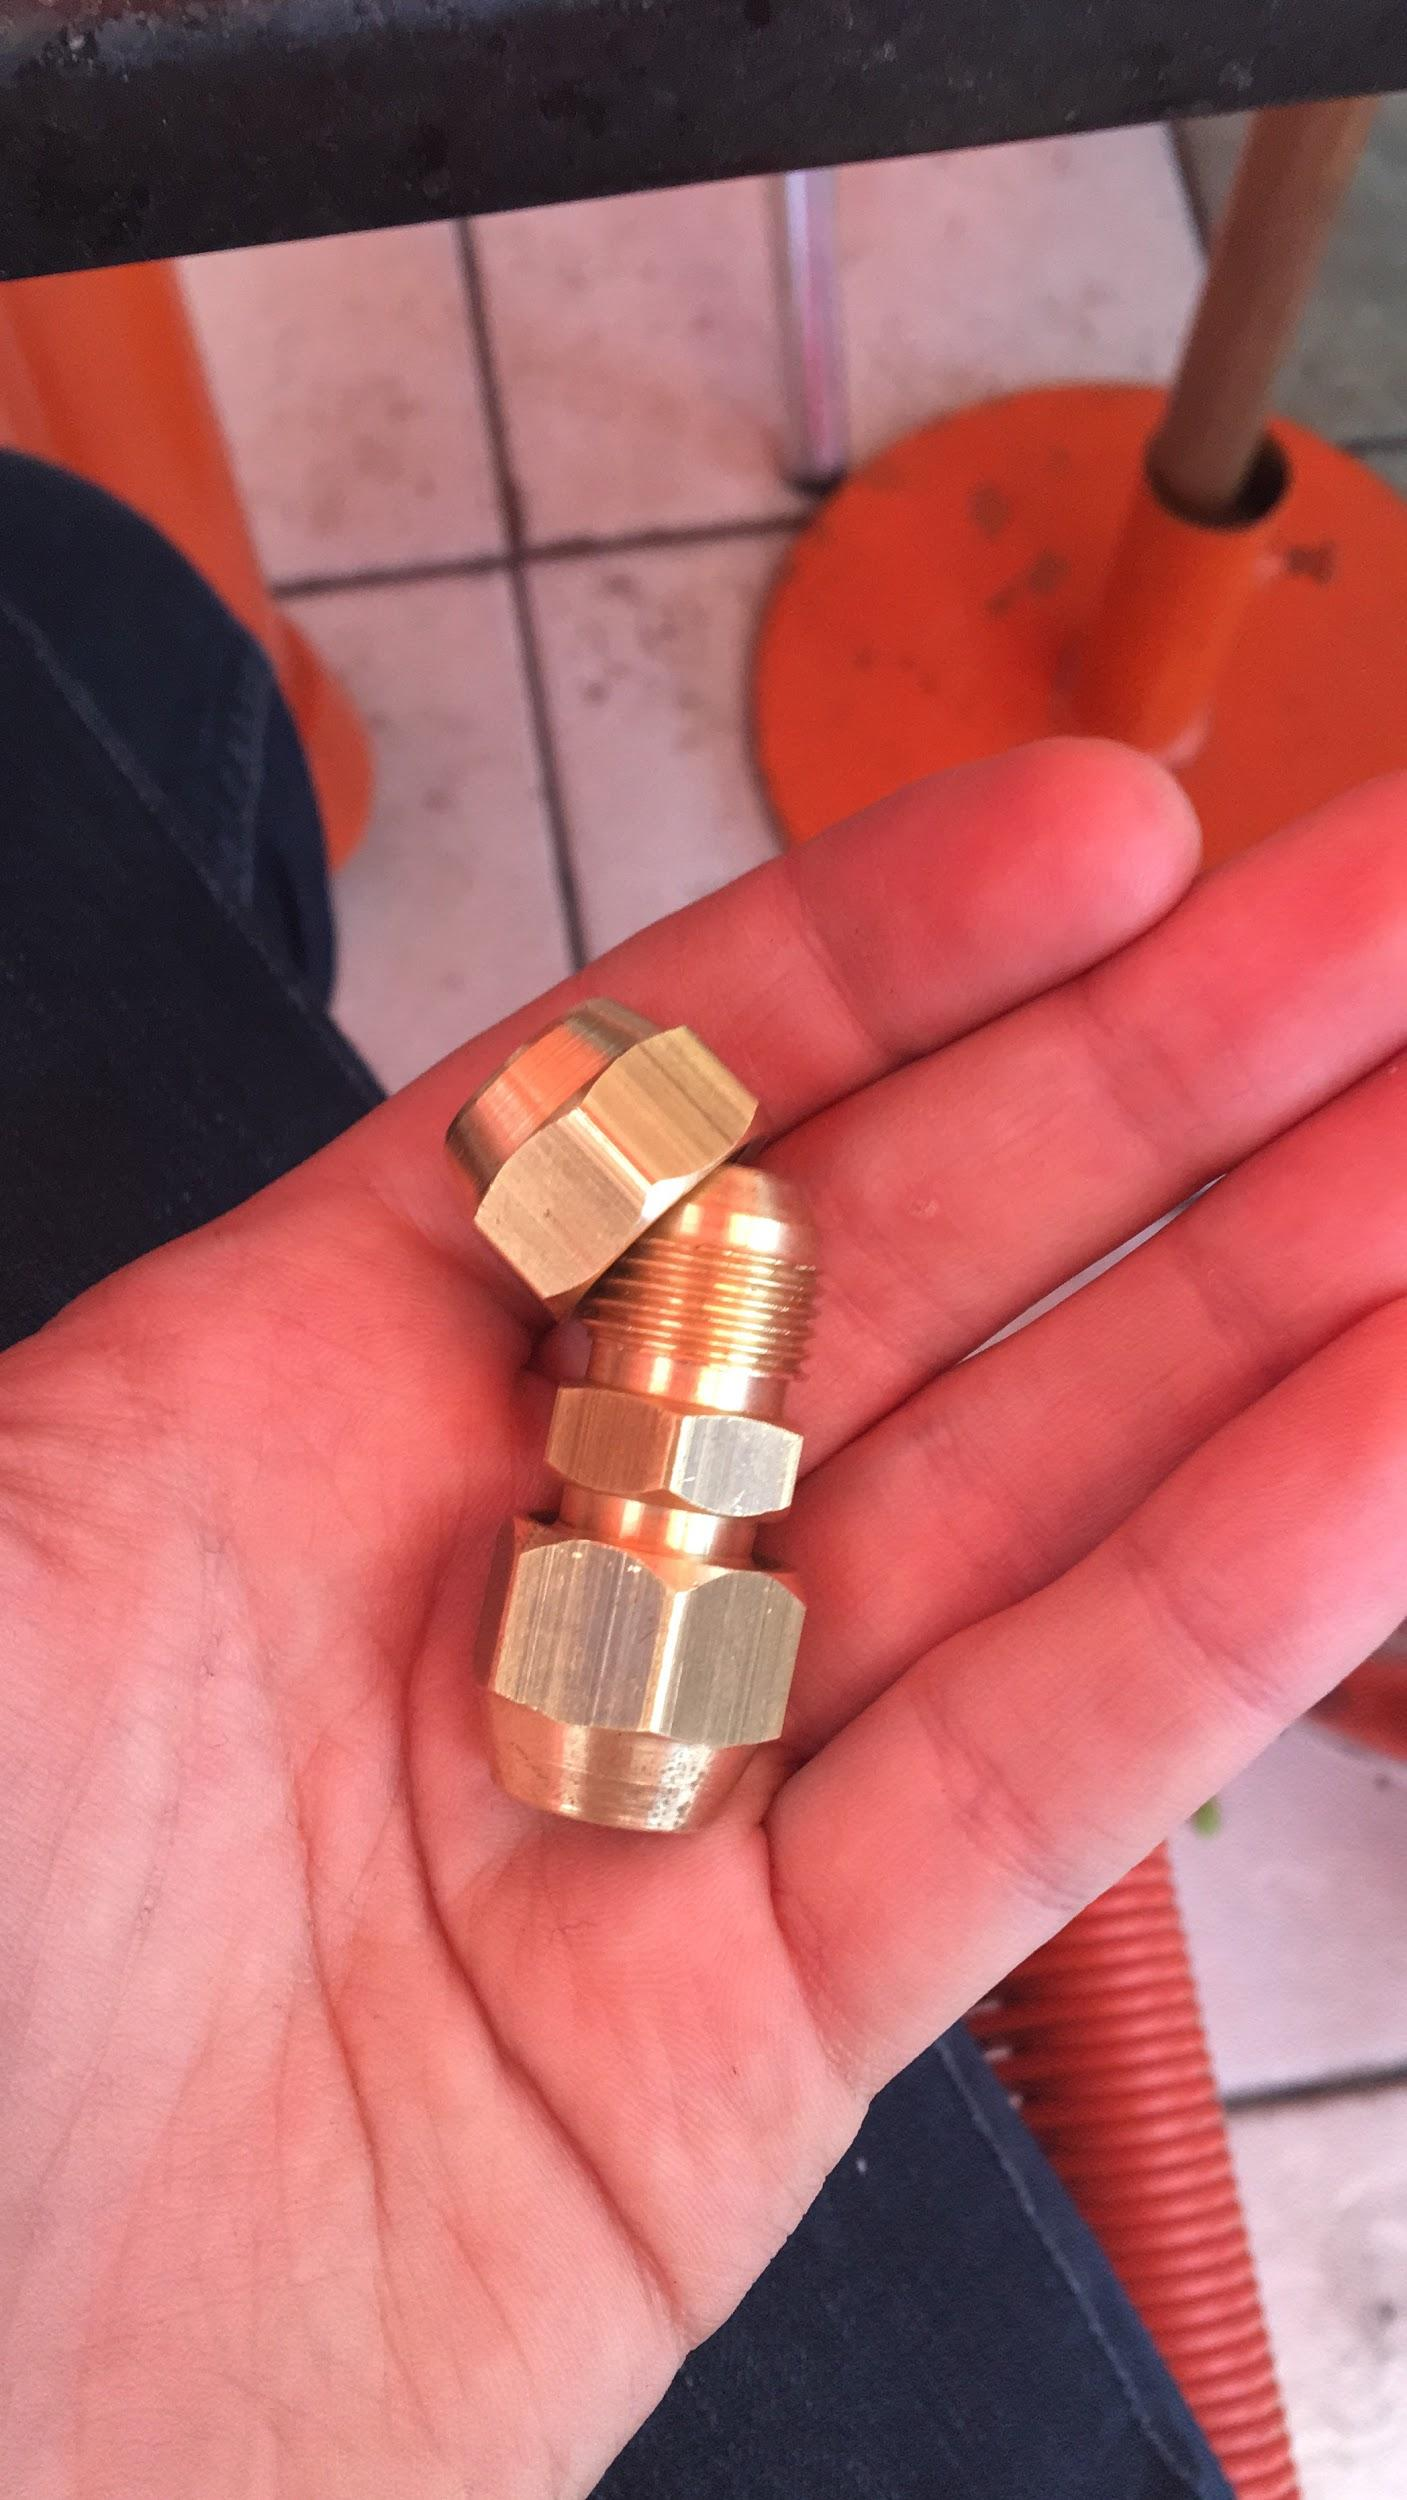
\includegraphics[scale= 0.2]{figuras/nipel-gas.png}
                    \caption{Nipel de gás. Fonte: Própria.}
                    \label{nipel-gas}
                \end{figure}

                Assim com a peça ilustrada na figura \ref{nipel-gas} realizou-se o processo de flangeamento dos
                tubos. Esse processo consiste em alargar a espessura do tubo de cobre para que o
                tubo de alumínio seja inserido e juntado pela peça acima não havendo vazamento de
                gás. O processo de flangeamento e ilustrado na figura \ref{processo-flageamento}.

                \begin{figure}[!htb]
                    \centering
                    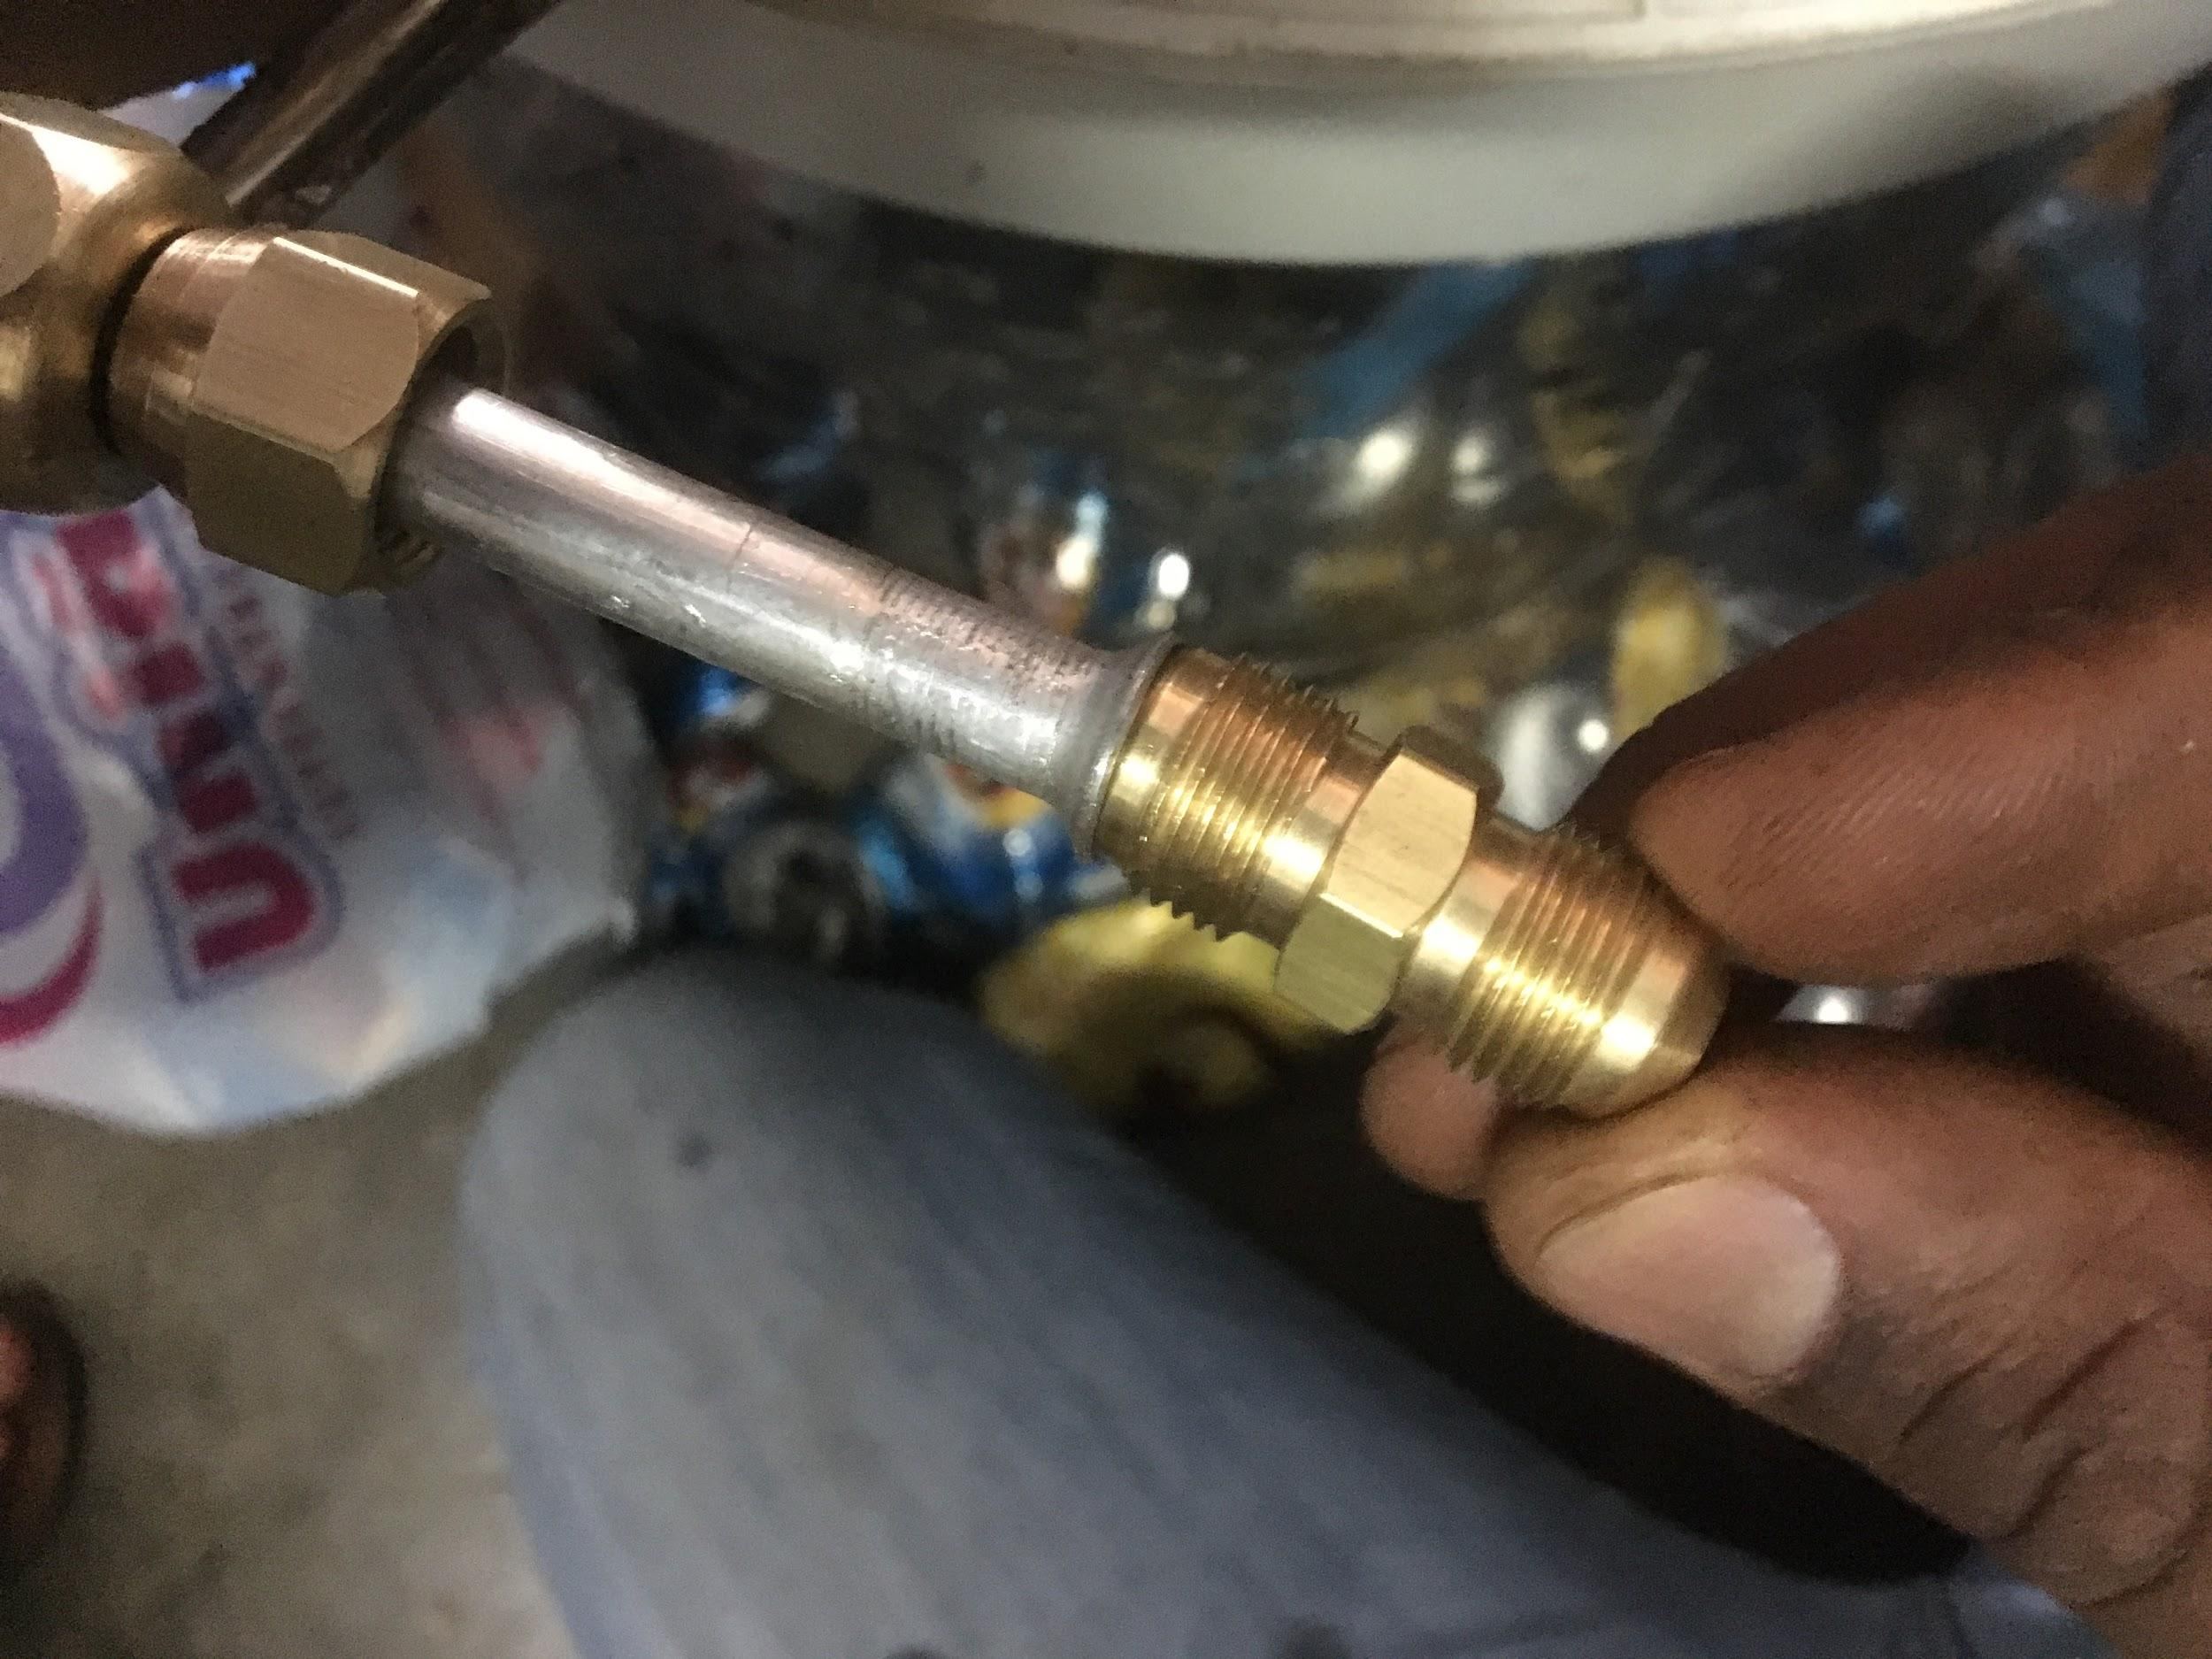
\includegraphics[scale= 0.2]{figuras/processo-flagelamento.png}
                    \caption{Processo de Flangeamento. Fonte: Própria.}
                    \label{processo-flageamento}
                \end{figure}
                
                \begin{figure}[!htb]
                    \centering
                    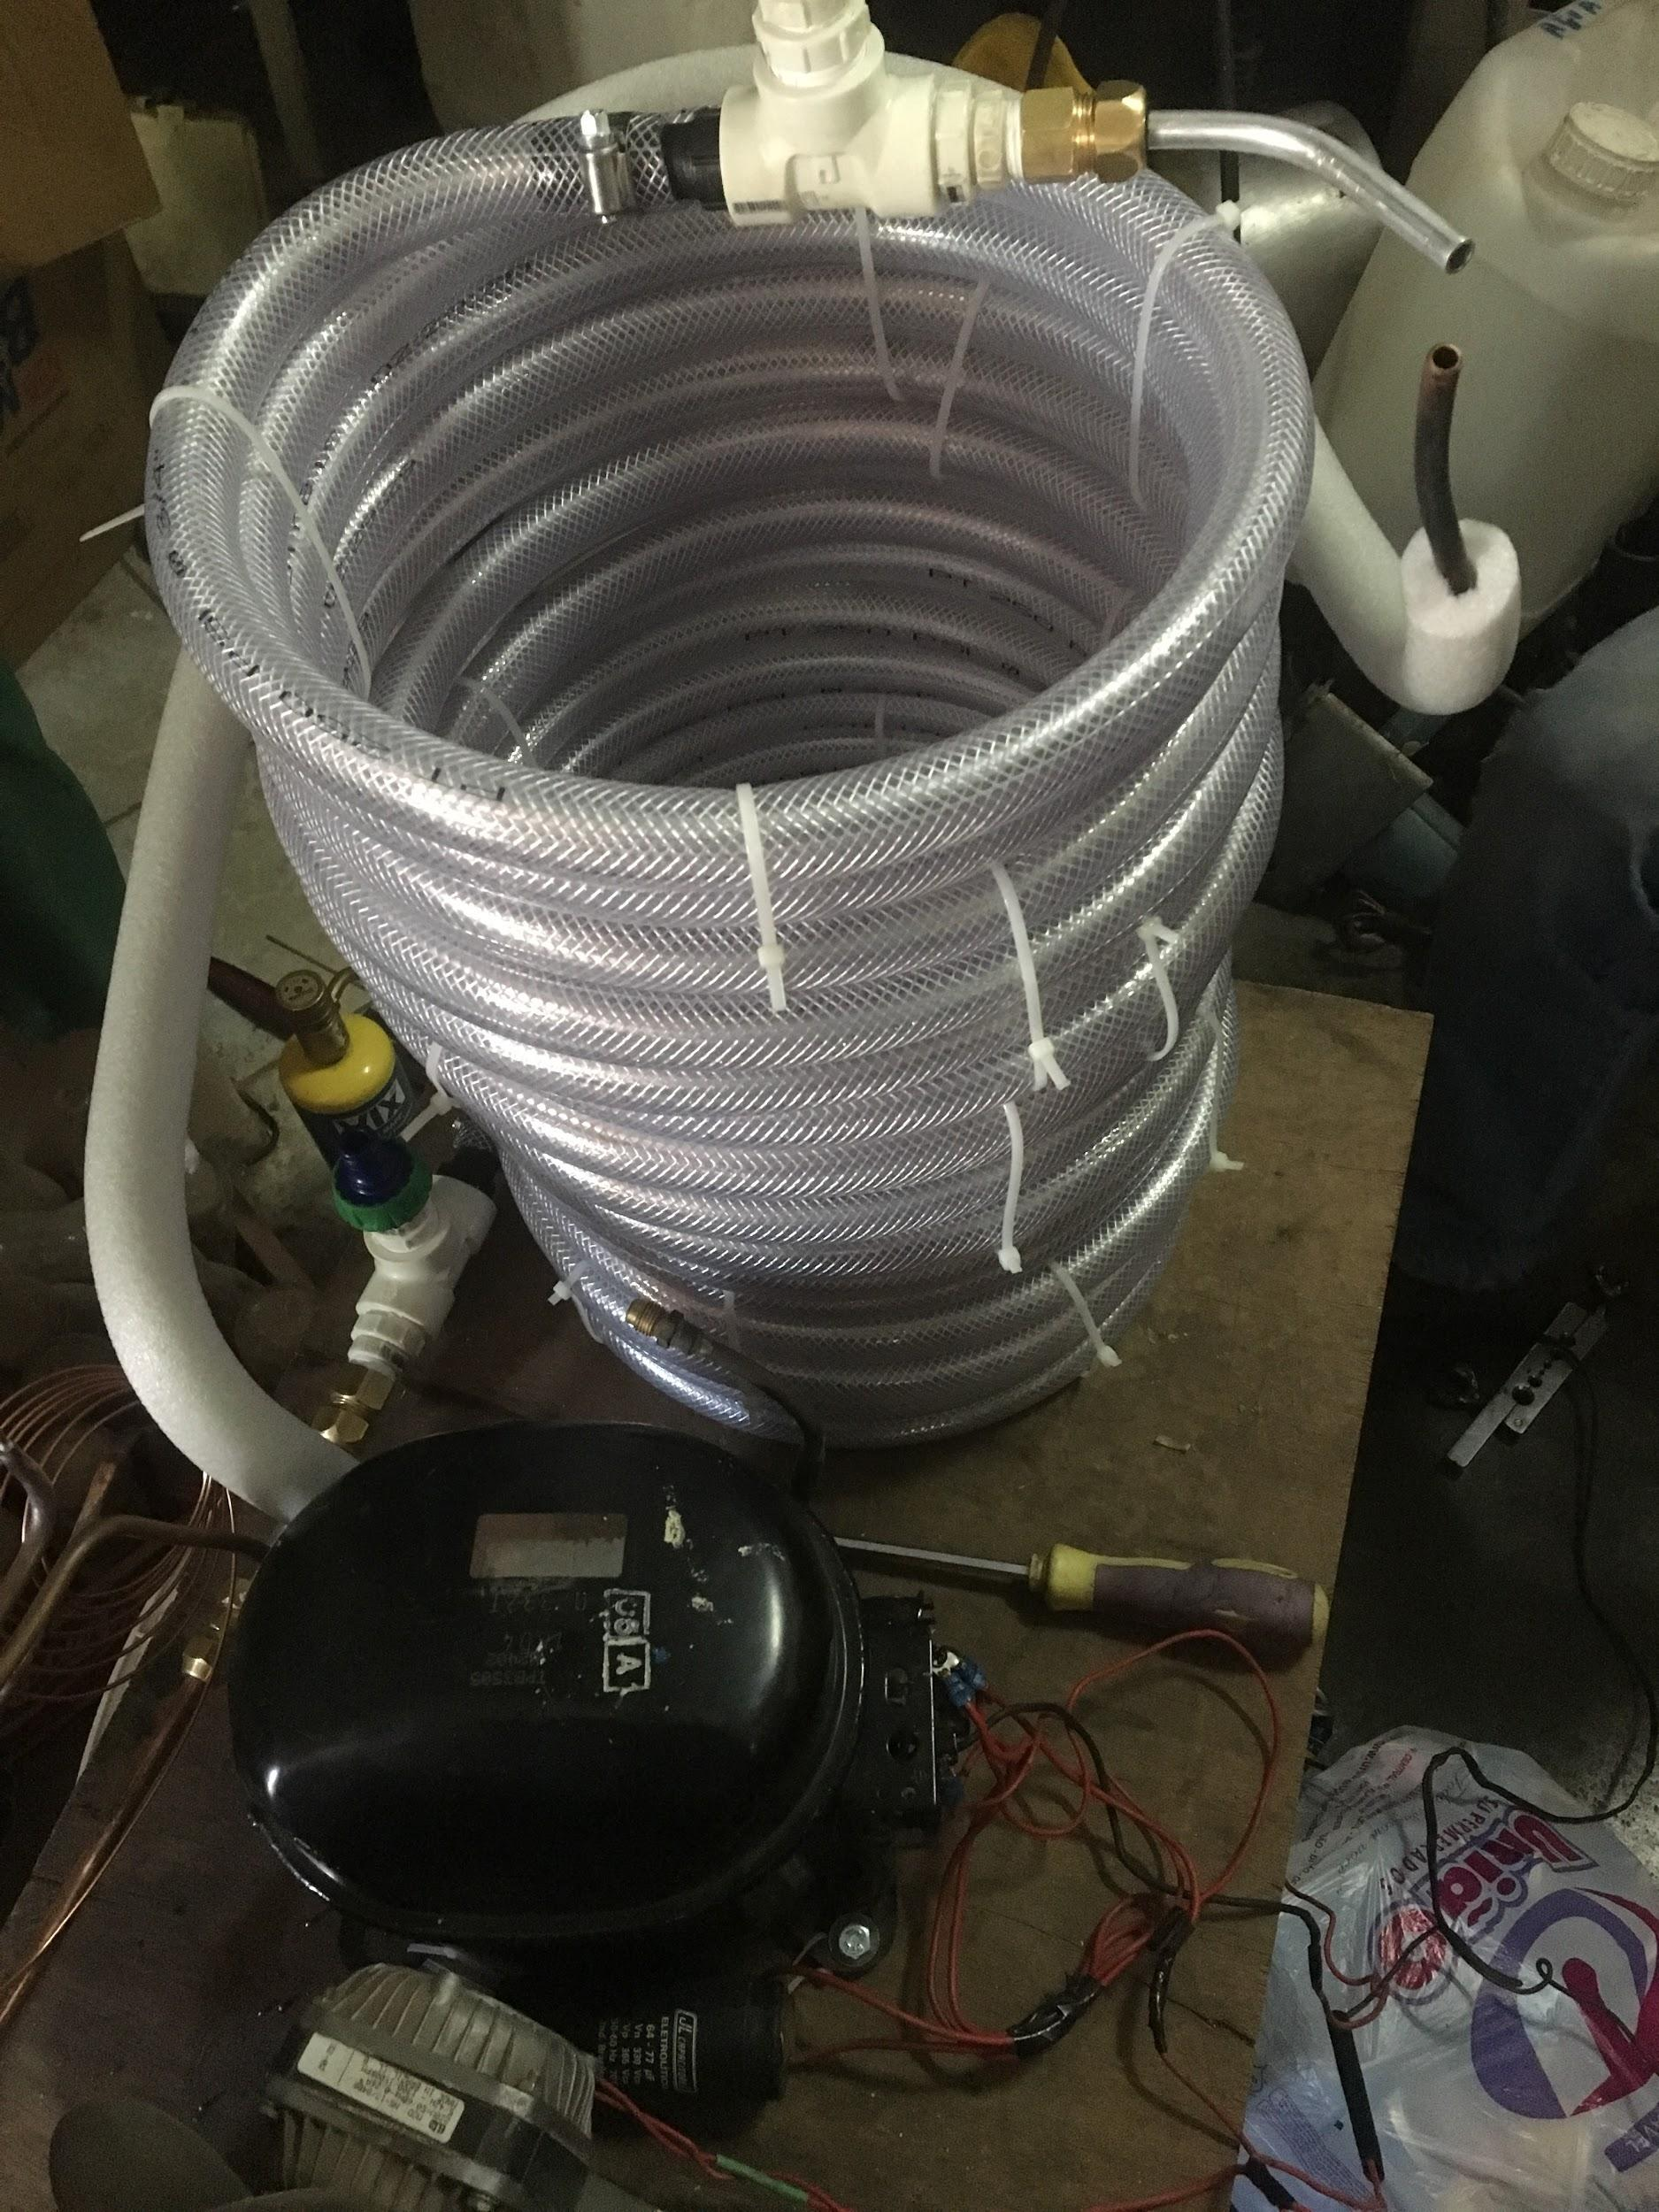
\includegraphics[scale= 0.2]{figuras/tubos-desconectados.png}
                    \caption{Tubos Desconectados. Fonte: Própria.}
                    \label{tubos-desconectados}
                \end{figure}

                Para a continuação da montagem do sistema, realizou-se a solda do tubo capilar
                e filtro secador. Assim, com o sistema todo soldado e montado foi feita a recarga de
                gás. Antes de abastecer o sistema, ligou-se o motocompressor para a realização de
                uma câmara de vácuo dentro das tubulações. Depois dessa verificação conectou-se o
                manifold nos diferentes pontos do sistema, parte de baixa e alta pressão e conectou-se
                a mangueira de abastecimento permitindo a passagem de fluido refrigerante. A carga
                foi realizada até que o sistema não suportasse mais gás dentro desse. A figura \ref{recarga-gas} mostra a recarga do sistema com o
                fluido refrigerante R22. 

                \begin{figure}[!htb]
                    \centering
                    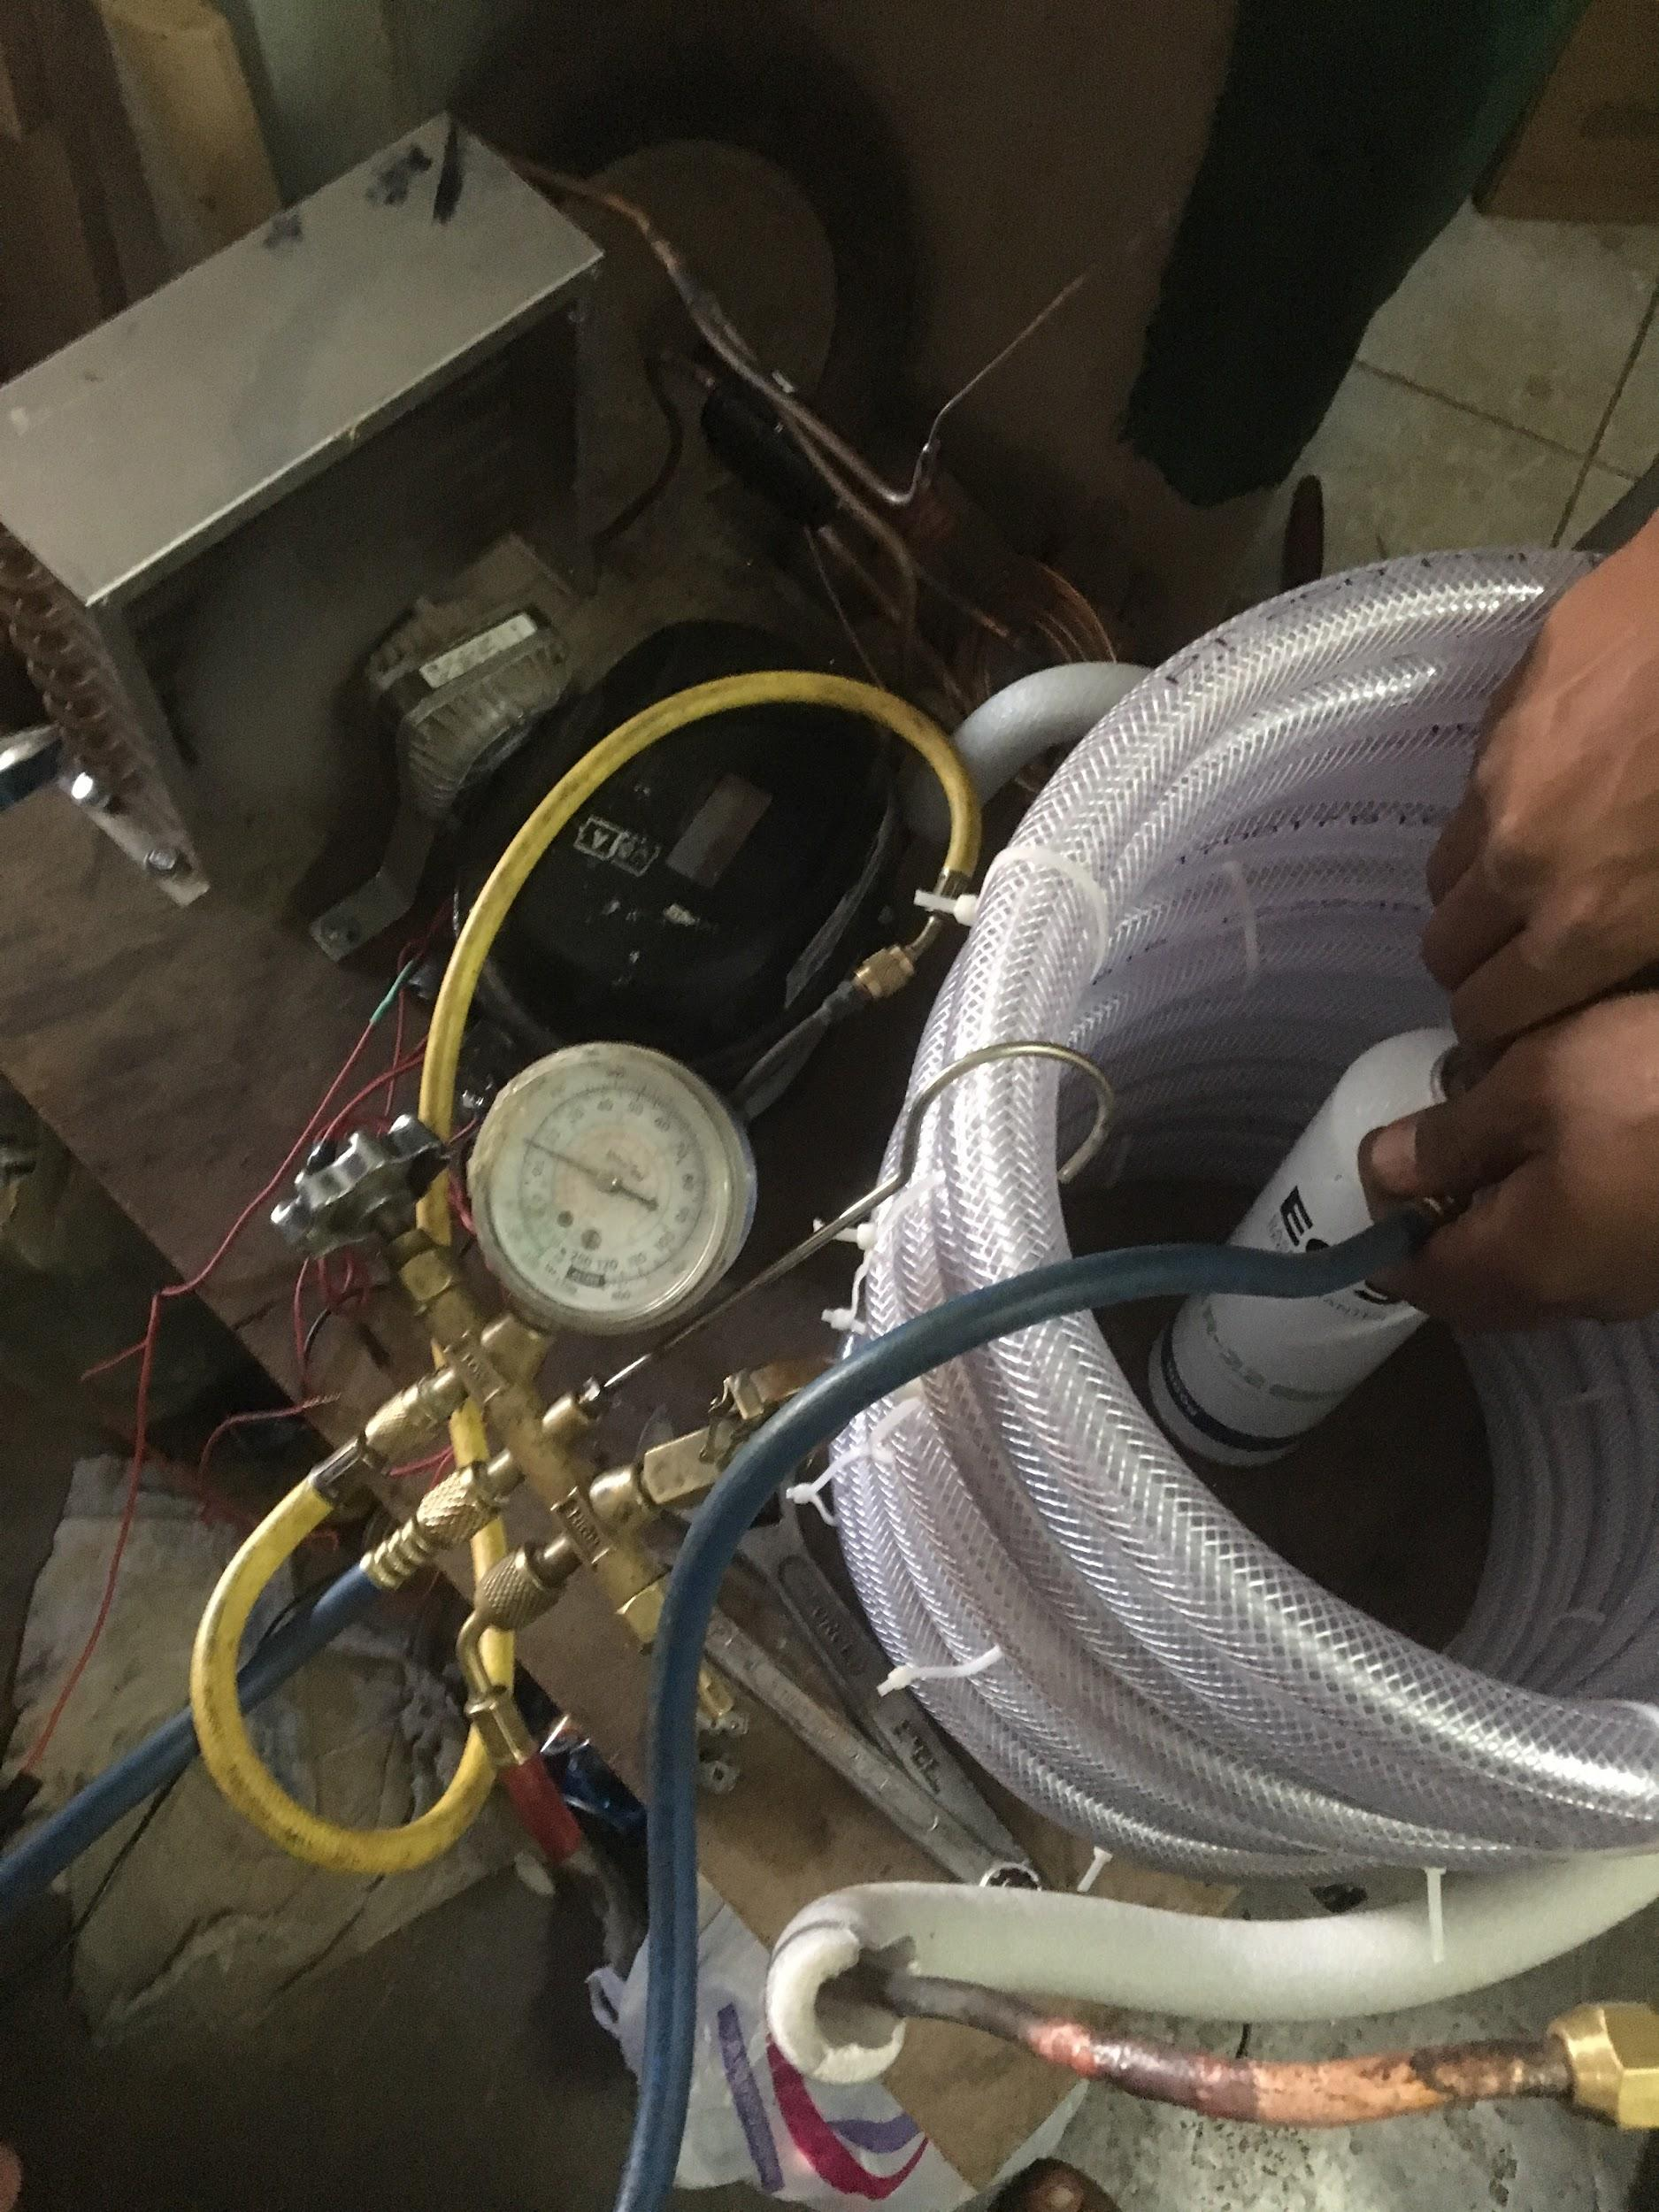
\includegraphics[scale= 0.2]{figuras/recarga-gas.png}
                    \caption{Recarga do sistema com gás R22. Fonte: Própria.}
                    \label{recarga-gas}
                \end{figure}

                Realizou-se os testes e notou-se que o condensador aplicado no sistema estava
                muito pequeno para o evaporador escolhido. Assim sendo, repetiu-se todos os passos
                acima quanto a soldagem dos tubos e a recarga de gás. Tendo assim o sistema de
                refrigeração da figura \ref{sistema-refrigeracao}.

                \begin{figure}[!htb]
                    \centering
                    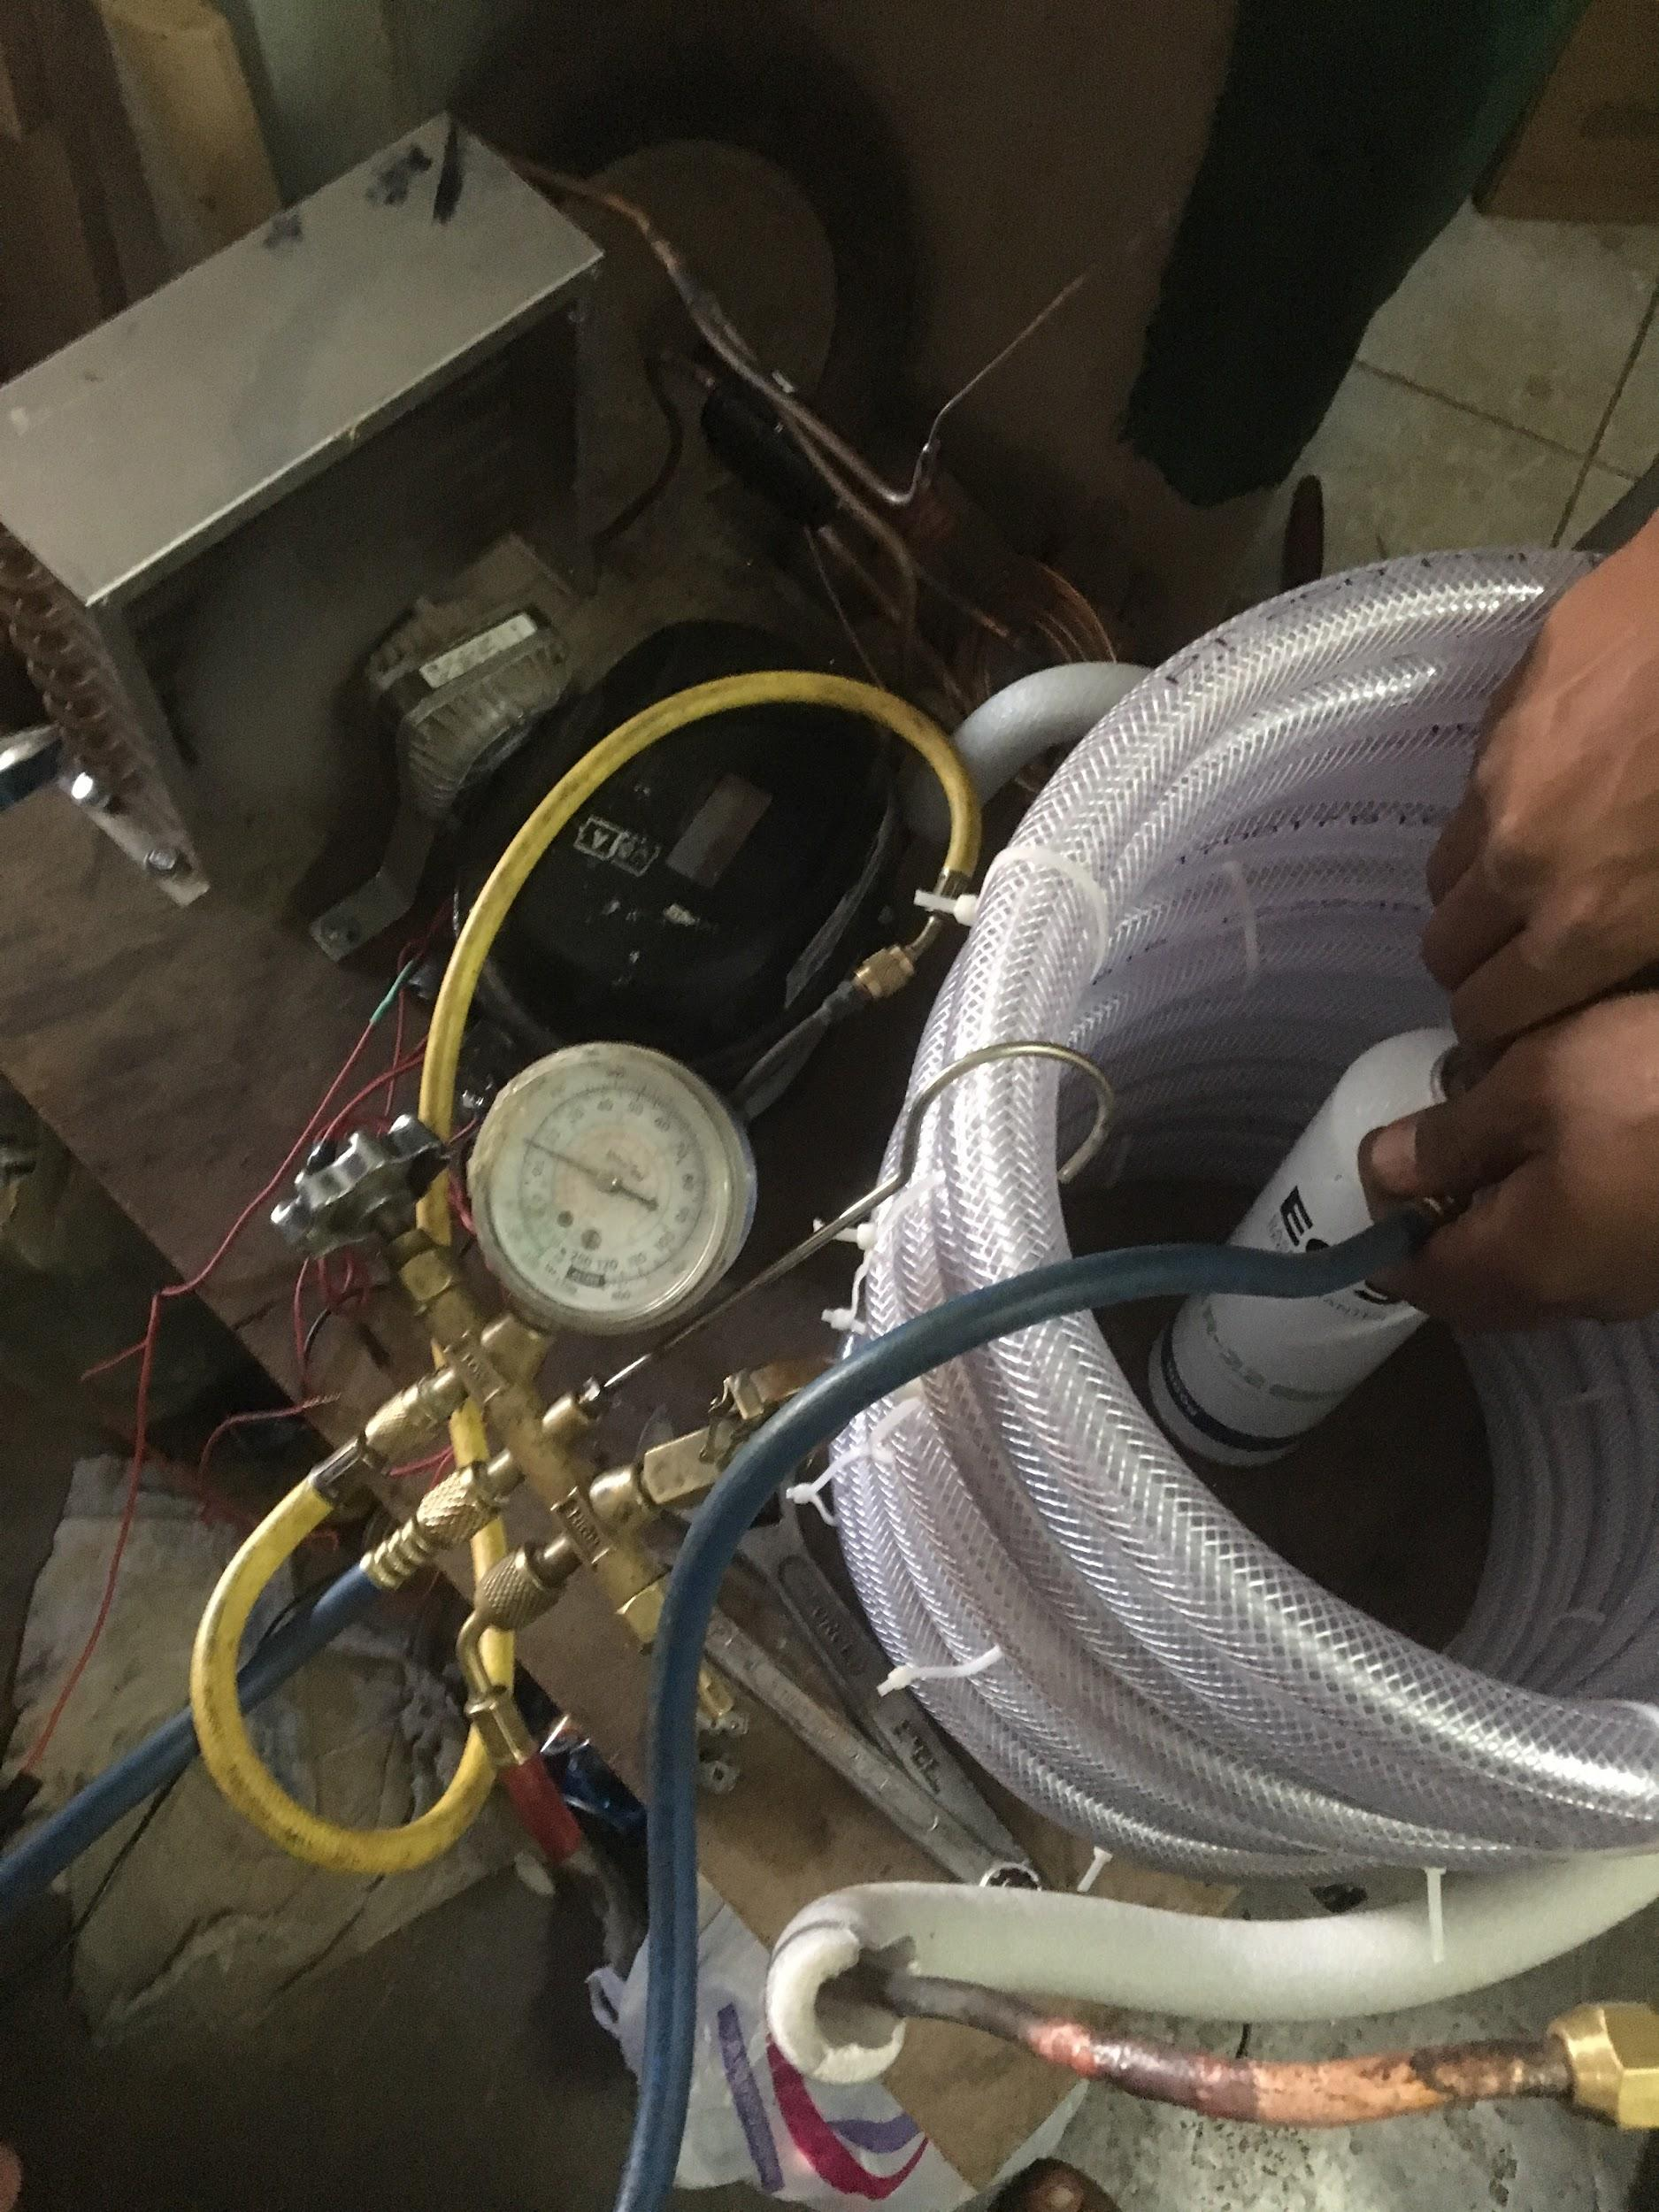
\includegraphics[scale= 0.2]{figuras/recarga-gas.png}
                    \caption{Sistema de Refrigreração. Fonte: Própria.}
                    \label{sistema-refrigeracao}
                \end{figure}

        \subsection[Casos de Teste]{Casos de Teste}
            \begin{itemize}
                \item \textbf{Componente} Chiller
                \item \textbf{Subsistema} Refrigeração
                \item \textbf{Pré-condição} Haver Chopp gelado
                \item \textbf{Entrada} Chopp quente
                \item \textbf{Saída} Chopp gelado
                \item \textbf{Fluxo de Eventos} Chopp quente entra em contra fluxo com o gás refrigerante a fim de
                    ter o chopp gelado.
            \end{itemize}

            Foi realizado um teste com o sistema de refrigeração pronto, adicionou-se água ao
            sistema, por onde deve-se entrar chopp. O motivo do teste ter sido feito com água
            antes, é que o aluguel ou compra de um barril de chopp é demasiadamente caro. Com
            o compressor ligado, colocou-se água no chirller de contra fluxo, para testar a troca de
            calor do mesmo. O resultado foi satisfatório, a água em uma temperatura ideal.

            \begin{table}[H]
                \centering
                \caption{Testes Iniciais do Sistema de Refrigeração}
                \label{testes-refrigeracao}
                \begin{tabular}{|l|l|}
                    \hline
                    Capacidade Efetiva de Chopp & 2,5 Litros \\ \hline
                    Tempo de Aquecimento do Sistema & 29 minutos \\ \hline
                    Tempo de Refrigeração &  20 - 37 minutos\\ \hline
                \end{tabular}
            \end{table}